\documentclass[11pt]{amsart}
\usepackage{geometry}                % See geometry.pdf to learn the layout options. There are lots.
\geometry{letterpaper}                   % ... or a4paper or a5paper or ... 
%\geometry{landscape}                % Activate for for rotated page geometry
%\usepackage[parfill]{parskip}    % Activate to begin paragraphs with an empty line rather than an indent
\usepackage{graphicx}
\usepackage{amssymb}
\usepackage{lscape}
\usepackage{booktabs}
\usepackage{caption}
\usepackage{longtable}
\usepackage{epstopdf}
\usepackage{verbatim}
\usepackage{rotating}
\usepackage{multirow}
\usepackage{multicol}
\usepackage{booktabs}
\usepackage{subfigure}

\usepackage{algorithm}
\usepackage{algpseudocode}
\DeclareGraphicsRule{.tif}{png}{.png}{`convert #1 `dirname #1`/`basename #1 .tif`.png}
\newtheorem{proposition}{Proposition}
\newtheorem{definition}{Definition}
\newcommand{\vertgeq}{\rotatebox{90}{$\leq$}}
\newcommand{\vertg}{\rotatebox{90}{$>$}}
\title{Draft}
\author{Lapo Santi}
%\date{}                                           % Activate to display a given date or no date

\begin{document}
\maketitle
%\section{}
%\subsection{}
\tableofcontents

\newpage

\section{Introduction}



When faced with a multitude of alternatives, individuals often strive to organize them into coherent blocks or groups to better understand the decision landscape. Furthermore, they aim to establish a meaningful order within these blocks, enabling them to prioritize alternatives based on preference. This process involves two fundamental tasks: block clustering and order-based ranking. While clustering involves categorizing alternatives into distinct blocks, ranking focuses on arranging these blocks in a specific order. These tasks are typically accomplished through human judgments, often in the form of pairwise comparisons.

In block clustering, the aim is to determine the inherent similarities among alternatives and group them accordingly. By comparing pairs of alternatives, individuals can identify common characteristics, shared attributes, or comparable features that contribute to their clustering. This process helps unveil the underlying structure of the alternatives, allowing decision-makers to comprehend the relationships and associations between them. Several techniques, such as hierarchical clustering and k-means clustering, have been employed to address this task effectively.

Conversely, in order-based ranking, the primary objective is to establish a preference-based order among the identified blocks of alternatives. By comparing pairs of blocks, individuals can discern the relative favorability of one block over another. These pairwise comparisons generate a ranking list that encapsulates the perceived preference or priority of each block. Various methodologies, including the Bradley-Terry model and pairwise comparison matrices, have been utilized to derive meaningful rankings from the collected preferences.

In this article, we propose a novel approach, termed Block Clustering and Order-based Ranking (BCOR), which unifies the tasks of block clustering and order-based ranking into a cohesive framework. The BCOR model introduces a dynamic parameter that governs the granularity of block clustering, allowing decision-makers to explore a spectrum of clustering options. By iteratively adjusting this parameter, the model can encompass a wide range of decision-making scenarios, from finely differentiated blocks to coarser groupings.

A key insight of the BCOR model lies in its ability to relate the number of blocks to the underlying ranking structure. As the number of blocks converges to the total number of alternatives, the model effectively transitions into a traditional ranking approach, providing a complete ordering of the alternatives. Conversely, by intentionally reducing the number of blocks, decision-makers are presented with distinct groups of choices, each requiring preference considerations within its own subset. This approach offers a nuanced perspective on decision-making, allowing individuals to differentiate between highly favored groups and those that are comparatively less preferred.

The BCOR model provides a flexible and adaptive solution for organizing and prioritizing alternatives in various decision-making contexts. Its application extends beyond conventional clustering and ranking tasks, empowering decision-makers to explore the continuum between comprehensive rankings and granular groupings. Additionally, the model can be tailored to incorporate different types of pairwise comparisons, enabling its utilization in diverse domains and decision scenarios.

To evaluate the effectiveness of the BCOR model, we conducted experiments using real-world datasets encompassing a wide range of decision contexts. The results demonstrate the model's ability to generate meaningful block clusters and order-based rankings, outperforming traditional approaches that solely focus on clustering or ranking tasks.

The contributions of this work can be summarized as follows:

We introduce the novel problem of block clustering and order-based ranking, bridging the gap between these two fundamental decision tasks.
We propose the BCOR model, which provides a unified framework to accommodate various levels of granularity in decision-making, from complete rankings to distinct preference-based groups.
We showcase the versatility of the BCOR model through experiments on real-world datasets, highlighting its superior performance compared to existing methods.
By integrating block clustering and order-based ranking, the BCOR model offers decision-makers a comprehensive tool to navigate complex decision landscapes




















\newpage



\section{The Simple Model}

The following Bayesian model is used to describe and analyze pairwise data, with the specific aim to identify clusters of points with similar connectivity patterns. Consider a scenario where entities engage in pairwise comparisons, and the outcomes are asymmetric – meaning that the probability of entity i winning over entity j is not necessarily the same as the probability of j winning over i. 


The model uses a Poisson distribution to model the number of blocks, a Dirichlet-multinomial distribution to model the distribution of nodes' assignment across blocks, and a binomial distribution to model the distribution of edges within blocks. Additionally, the model includes a POMM process to model the probability of edge formation between nodes within blocks.

The goal of the model is to estimate the number of blocks, the distribution of nodes across blocks, and the probability of edge formation between nodes within blocks, given observed network data. The Bayesian approach allows for uncertainty in these estimates and provides a framework for incorporating prior knowledge and updating beliefs as new data becomes available.

\subsection{Simple Model specification}
This is a model for pairwise count data. We explicitly model the results of the interactions between two individuals $i$ and $j$. Given $N$ observations, the likelihood is 
\begin{align}
p(y| z, P, K) &= \prod_{i =2 }^{N-1} \prod_{j =i}^{N} p(y_{ij} | z, P, K) \\ 
&= \prod_{i =2 }^{N-1} \prod_{j =i}^{N}  {n_{ij} \choose y_{ij}} p_{z_i, z_j}^{y_{ij}}(1- p_{z_i, z_j})^{n_{ij}-y_{ij}}
\end{align}

where $n_{ij}$ denotes the total number of interactions between the two individuals $i$ and $j$ and $y_{ij}$ is the number of successes of the individual $i$ in interacting with $j$. The probability of success is given by $p_{z_i, z_j}$ which consists of two parameters. The $K\times K$ matrix $P$ and the $N \times 1$ vector $z$.

The vector $z$ takes values over the discrete and finite set $\{ 1 , \ldots, K\}$, and it is an indicator variable such that if $z_i = k$ individual $i$ belongs to block $k$. 

The matrix $P$ contains the probabilities of success for individuals belonging to each possible blocks combination. For this reason $P$ is $K\times K$. Therefore, the parameter $p_{z_i, z_j}$ consists in the probability of success in an interaction between one individual belonging to block $z_i$ and another of block $z_j$. 

\subsection{Prior Specification}

This model has three parameters, and we put a prior on each of them.

Starting with $P$, we assume that its entries, namely $p_{k,k^\prime}$, are independent and identically $Beta(a,b)$ distributed random variable. By setting $a=b=1$ they collapse to a uniform distribution.
\begin{equation}
p_{k,k^\prime} \sim Beta(1,1) \quad \text{for } k,k^\prime = 1, \ldots,K
\end{equation}
Second, we assume that the $z_i$s are independent and identically drawn from a multinomial distribution with one trial and probability vector $(\theta_1, \dots, \theta_K)$. We can write then:
\begin{equation}
z_i| \boldsymbol{\theta} \sim \operatorname{Multinomial}(1,\boldsymbol{\theta}) \quad \text{for } i = 1, \ldots,N
\end{equation}


To have more flexibility in the blocks sizes, we put an hyper-prior on the $\theta_1, \dots, \theta_K$, assuming that they are drawn from a Dirichlet distribution with parameter the $K\times1$ vector $\boldsymbol{\gamma}$.


By marginalizing out $\theta$, following the common practice in the literature, we can express the marginal distribution of $z$ as:

\begin{equation} p(\mathbf{z}|\boldsymbol{\gamma}) = \frac{\Gamma(\sum_{k=1}^K \gamma_k)}{\prod_{k=1}^K \Gamma(\gamma_k)}\frac{\prod_{k=1}^K \Gamma(n_k+\gamma_k)}{\Gamma(\sum_{k=1}^K (n_k+\gamma_k)}
\end{equation}

where $n_k$ is the number of players assigned to block $k$.

Finally, we assume that the number of clusters $K$ follow a Poisson distribution $\operatorname{Poisson}(\lambda=1)$, subject to the condition $K>0$.


\clearpage

\section{The POMM Model}



In this section, we introduce a novel pairwise model that combines the notions of ordering and community structure to capture the complex interactions observed in various systems. Just as in network analysis, where directed hierarchies and community patterns play crucial roles in understanding interactions among entities (see Peixoto), we seek to develop a framework that simultaneously incorporates these two fundamental aspects in the context of pairwise data.


Drawing inspiration from the directed stochastic block model (SBM) used in network analysis, we develop a modified version tailored specifically for pairwise data. The model allows us to identify directed hierarchies among the entities while simultaneously detecting community structures that influence their interactions. By incorporating these two elements into a unified framework, our model offers a more comprehensive understanding of the underlying dynamics governing pairwise comparisons.

Several models of stochastic transitivity exist and have been used to describe the probabilities involved in experiments of paired comparisons, specifically in scenarios where transitivity is expected, however, empirical observations of the binary relation is probabilistic. This allows for a weaker player to win with a positive probability against a stronger opponent. 

Tightly matched players might have a higher chance of observing this inversion while players with large differences in their skills might only see these inversions happen seldom. Stochastic transitivity models formalize such relations between the probabilities (e.g. of an outcome of a match) and the underlying transitive relation (e.g. the skills of the players).

Tightly matched players might have a higher chance of observing this inversion while players with large differences in their skills might only see these inversions happen seldom. Stochastic transitivity models formalize such relations between the probabilities (e.g. of an outcome of a match) and the underlying transitive relation (e.g. the skills of the players).

A binary relation $\succsim$ on a set $\mathcal{A}$ is called \emph{transitive}, in the standard \textit{non-stochastic} sense, if
$a \succsim b$ and $b \succsim c$ implies $a \succsim c$ for all members $a,b,c$ of $\mathcal{A}$.

\emph{Stochastic} versions of transitivity include:
\begin{enumerate}
  \item \textbf{Weak Stochastic Transitivity (WST):} $\mathbb{P}(a\succsim b)\geq \tfrac{1}{2}$ and $\mathbb{P}(b\succsim c)\geq \tfrac{1}{2}$ implies $\mathbb{P}(a\succsim c)\geq \tfrac{1}{2}$, for all $a,b,c \in \mathcal{A}$;
  \item \textbf{Strong Stochastic Transitivity (SST):} $\mathbb{P}(a\succsim b)\geq \tfrac{1}{2}$ and $\mathbb{P}(b\succsim c)\geq \tfrac{1}{2}$ implies $\mathbb{P}(a\succsim c)\geq \max \{\mathbb{P}(a\succsim b),\mathbb{P}(b\succsim c)\}$, for all $a,b,c \in \mathcal{A}$;
  \item \textbf{Linear Stochastic Transitivity (LST):} $\mathbb{P}(a\succsim b) = F(\mu(a) - \mu(b))$, for all $a,b \in \mathcal{A}$, where $F:\mathbb{R} \to [0,1]$ is some \textit{increasing} and symmetric function (called a \emph{comparison function}), and $\mu: \mathcal{A}\to \mathbb{R}$ is some mapping from the set $\mathcal{A}$ of alternatives to the real line (called a \emph{merit function}).
\end{enumerate}

In the following sections we will focus on the Strong Stochastic Transitivity version.

\subsection{Assuming the SST property for the probabilities in matrix P (SST matrix)}
Starting from the Simple model, we modify the parameter $P$, so that it satisfies the SST assumption. Recall that $\underset{K \times K}{P}$ is a collection of victory probabilities among $K$ blocks or communities as follows:

\begin{center}
$$P = 
\left(\begin{array}{cccc}p_{1,1} & p_{1,2} &  ... & p_{1,K} \\ p_{2,1} & p_{2,2} & ... & p_{2,K} \\ \vdots & \vdots & \vdots & \vdots \\ p_{K,1}& p_{K,2 }& ... & p_{K,K}\end{array}\right)$$
\end{center}


In order to satisfy the SST property, P entries can be spelled out explicitly as follows:
\begin{center}
$$
\left(\begin{array}{ccccccc} 0.5 & \leq & p_{1,2} & \leq &  ... & \leq & p_{1,K} \\  &  & \vertgeq &  & ... &  & \vertgeq \\
1 - p_{1,2} & \leq & 0.5 & \leq & ... & \leq & p_{2,K} \\ \vdots & \vdots & \vdots & \vdots &  ... & \vdots& \vdots \\ 1 - p_{1,K}& \leq & 1 - p_{2,K}& \leq & ... & \leq & 0.5\end{array}\right)
$$
\end{center}

We further assume that the P matrix is skew-simmetric, that is, $p_{j,i}= 1 - p_{i,j}$. Furthermore, we set the main diagonal of matrix $P$ to $0.5$ for teams and $0$ for individual players.

\begin{figure}
\begin{center}
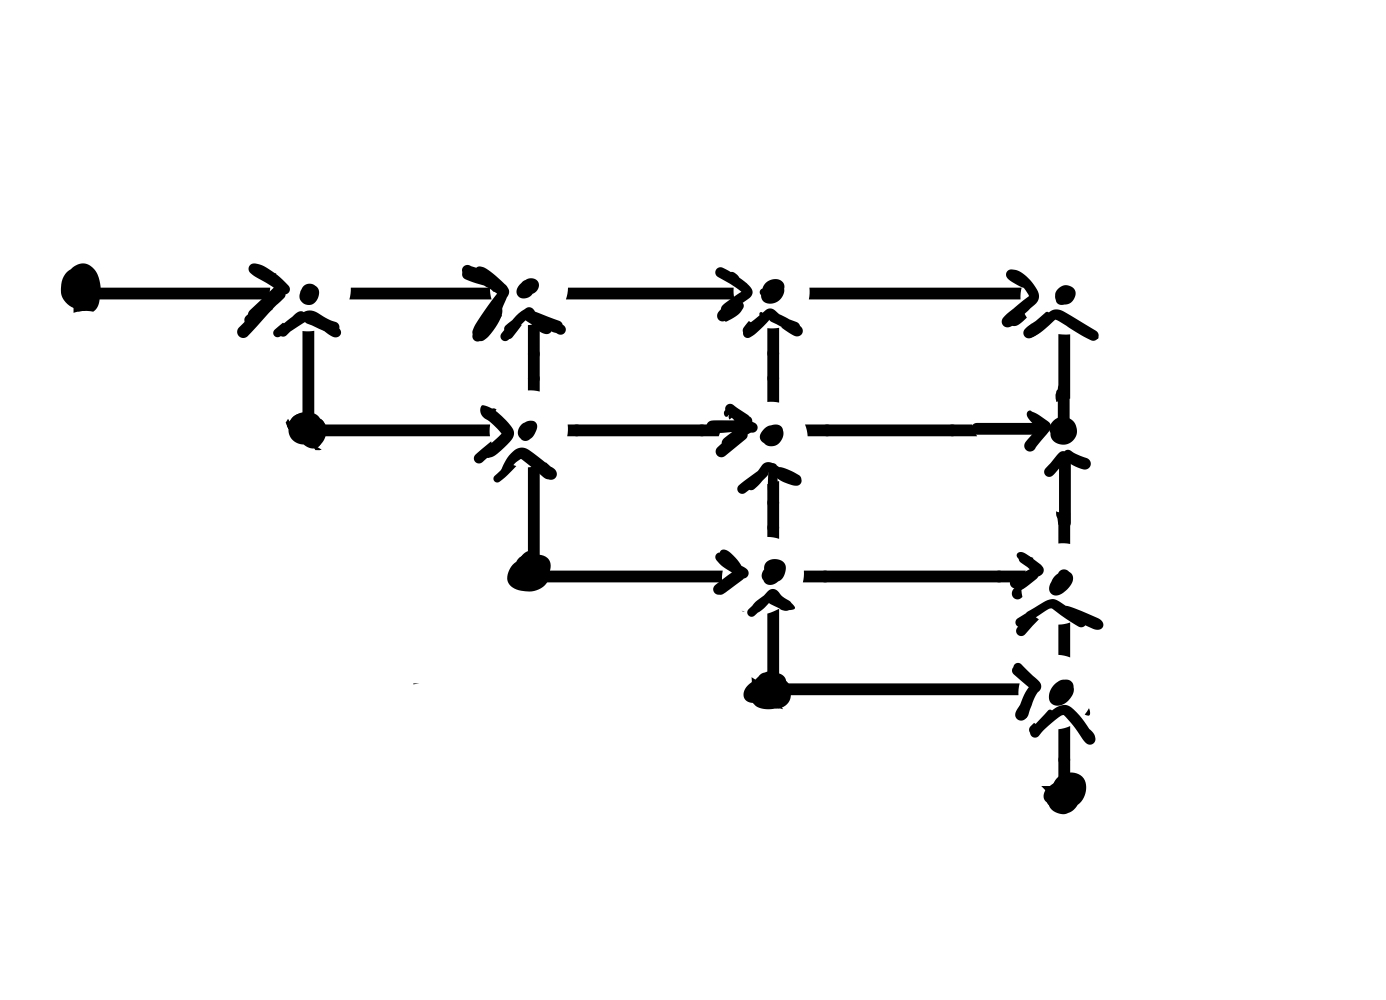
\includegraphics[width=0.6\textwidth,natwidth=1386,natheight=1000]{/Users/lapo_santi/Desktop/Nial/project/POMMs/IMG_0EE4E8AB347D-1.jpeg}
\caption{Dag representation of the Poset imposed onto the SST matrix}
\label{fig:DAG}
\end{center}
\end{figure}


\subsection{Prior on $P$}

In order to incorporate such structure within a Bayesian framework, we need to impose an appropriate prior and hyper-prior on $P$ so to reproduces such ordering among the probabilities. To this end, we draw inspiration from the the literature on spatial statistics. In particular, we exploit the idea of Partially Order Markov Models (POMMs) to define dependency and structure within the $P$ matrix. 

\subsection{Posets and Dags}
 $P$ is a partially ordered set (Poset) $(P, \leq)$ where a Poset is defined as follows.

\begin{definition}\label{def:Poset}[Poset]A poset, a partially ordered set, is a set of elements $D$ where a binary relation $\prec$ defined on $D$ itself is such that:
\begin{align}
&\text{For any } x \in D, x \prec x (\text{ reflexivity }) \\
&\text{For any } x,y,z \in D, x \prec y \text{ and } y \prec z \implies x \prec z (\text{ transitivity }) \\
&\text{For any } x, y \in D, x \prec y \text{ and } y \prec x \implies x = y (\text{ antisymmetry }).
\end{align}
Then we call $(D, \prec)$ a partially ordered set, or a \textit{poset}. 
\end{definition}

We see that $(P, \leq)$ satisfies the three properties of Definition \eqref{def:Poset}, and therefore, is a poset. Let us now explicit how posets can be represented using directed cyclic graphs; we will see later how this will turn out useful to elicit the dependency structure between $P$'s elements.

Let us denote with $(V, E)$ the vertex and the edge sets of be a directed acyclic graph, respectively. To find the pair $(V=P, E)$, meaning the graph corresponding to the poset $P$, we define the edge set $E$ so that every pair $\{(p_i, p_j) \in E \} \implies p_i \leq p_j$.

This correspondence is many-to-one. Given a finite poset, one may construct a class of directed acyclic graphs; however, it may be of particular interest the minimal directed acyclic graph since it has the smallest possible directed edge set, which consists in $\{(p_i, p_j) \in E \} \implies p_i \leq p_j \land \{p_k : p_i\leq p_k\leq p_j \} = \emptyset \}$

We represent the minimal directed acyclic graph $(P, E)$ corresponding to $P$ in figure (\ref{fig:DAG}) by using the definition of Adjacent Lower Neighborhood that we introduced before.


\begin{definition}[Cone]
For any $y \in D$, the \textit{cone} of $y$ is the set
\begin{equation}
\text{ cone } y = \{x \in D: x\prec y;x\neq y \} \nonumber
\end{equation}
\end{definition}

\begin{definition}[Adjl]
For any $y \in D$ the \textit{adjacent lower neighbourhood} of $y$ is the set $$
\text{adjl } y = \{ x \in D:(x,y) \text{is a directed edge in} (D,F)\}
$$
\end{definition}




\begin{definition}[Cover of a Subset]
The cover of a subset $B$ is a set of all elements $x$ in $D$ such that $x$ is adjacent to an element in $B$ and $x$ is not in $B$. Formally, the cover of $B$ is defined as follows:
\begin{equation}
\text{covr}\ B = { x \in D: \text{adjl}\ x \subset B \text{ and } x \notin B } \nonumber
\end{equation}
where $\text{adjl}\ x$ is the set of all adjacent elements of $x$ in $D$.
\end{definition}
Intuitively, the cover of a subset $B$ represents all the elements in $D$ that are outside of $B$ but are adjacent to at least one element in $B$. In other words, the cover of $B$ captures the neighborhood of $B$ in $D$.

\begin{definition}[Level Sets]
The level sets of a poset $D$ are a sequence of nonempty cover sets defined recursively as follows:
\begin{equation}
L^0 = D_{min};\quad L^i = \text{covr}\left( \bigcup_{k=0}^{i-1} L^k \right) \nonumber
\end{equation}
where $D_{min}$ is the set of all minimal elements in $D$.
\end{definition}

The first level set $L^0$ is simply the set of all minimal elements in $D$. The subsequent level sets are defined by taking the union of all the previous level sets and taking the cover of this union. Intuitively, each level set captures the neighborhood of the previous level sets in $D$.



\subsection{Partially ordered Markov models:}

Consider a finite set of random variables $\{ Z(s_1),\ldots,Z(s_n) \}$ indexed by location or "points" $$
D = \{s_1,\ldots ,s_n \}: n \in \{1,2,\ldots \}
$$

That is, we assume the existence of a directed acyclic graph $(D,F)$ and its corresponding poset $(D,\prec).$
Let $(D,F)$ be a finite, directed acyclic graph and its corresponding poset $(D,\prec).$ Consider $s \in D$ and recall the definition of cone $s$. Also, let the quantity $U_s$ denote any subsets of points not related to s. 
Formally:
$$
U_s \subset \{ u \in D: u \text{ and } s \text{ are not related } \}
$$
\begin{definition}[POMM]
Then $\{ Z(s): s \in D \}$ is said to be a partially ordered Markov model (POMM) if , for all $s \in D$ and any $U_s$
\begin{equation}
P(Z(s)|Z(\text{ cone } s), Z(U_s)) = P(Z(s)|Z(\text{ adjl } s)
\end{equation}
\end{definition}
\begin{proposition}\label{eq:result1}[Joint Distribution]
Let $(D,F)$ be a directed acyclic graph with no singleton points and let $(D, \prec)$, be its associated poset. Suppose that $\{Z(s): s \in D\}$ is a POMM. Then 
\begin{align}
P(Z(D)) &= P(Z(L^0)) \prod_{k=1}^m \prod \{ P(Z(u))| Z(\text{ adjl } u): u \in L^k \} \\
&= P(Z(L^0)) \prod \{ P(Z(u))| Z(\text{ adjl } u): u \in D 
\setminus L^0 \}
\end{align}
where $L^0, L^1, \ldots L^m$ are the level sets as defined previously.
\end{proposition}







Result 1 relates the probability of a random variable defined on a poset to the probabilities of its restrictions to the lower level sets of the poset.

The result states that the probability of $Z$ on the entire poset $D$ can be expressed as a product of the probabilities of $Z$ restricted to the level sets $L^0, L^1, \ldots, L^m$ of the poset, where $L^0 = D_{\text{min}}$ is the set of minimal elements of $D$, and $L^k$ is the set of elements of $D$ that are not in any of the previous level sets $L^0, L^1, \ldots, L^{k-1}$ and whose immediate predecessors are all in the union of the previous level sets $\bigcup_{i=0}^{k-1} L^i$.

The first part of the result states that the probability of $Z$ on $D$ is equal to the product of the probability of $Z$ on $L^0$ and the conditional probabilities of $Z$ on the elements of each subsequent level set $L^k$, given the values of $Z$ on their immediate predecessors. This can be seen as a form of the chain rule of probability, where the joint probability of $Z$ on $D$ is decomposed into a product of conditional probabilities.

The second part of the result simplifies the product by noting that the conditional probabilities of $Z$ on the elements of $D\setminus L^0$ are determined by the values of $Z$ on their immediate predecessors, which are all in $L^0$ or $D\setminus L^0$. Therefore, the product can be simplified to the product of the probability of $Z$ on $L^0$ and the conditional probabilities of $Z$ on the elements of $D\setminus L^0$ given the values of $Z$ on their immediate predecessors in $D\setminus L^0$. This simplification reduces the number of terms in the product and makes the computation of the joint probability of $Z$ on $D$ more efficient.




\newpage







\section{Application to the SST matrix}




In this section, we introduce a matrix that exhibits the Strong Stochastic Transitivity (SST) property. Our aim is to model the probabilities of players winning matches in a tournament, ensuring that these probabilities are consistent. Transitivity, as mentioned above, is crucial in guaranteeing that if Player A is stronger than Player B and Player B is stronger than Player C, then Player A must be stronger than Player C. This logical relationship is reflected in the probabilities of victory between players, which are contained in the matrix $P$ introduced in the previous section.
The matrix under consideration is denoted as $\underset{K \times K}{P}$, representing victory probabilities among $K$ entities, such as players or groups of players. Each element $p_{i,j}$ in the matrix $P$ represents the probability of player $i$ winning against player $j$ in a tennis match, without draws allowed. To satisfy the requirements of a valid probability, we have $p_{i,j} + p_{j,i} = 1$, where $p_{j,i} = 1 - p_{i,j}$.

Without loss of generality, we assume that player/team 1 is the strongest and player/team $K$ is the weakest. Monotonicity in the probabilities is crucial, ensuring that the probabilities increase monotonically as the index of the columns $j$ increases and decrease monotonically as the index of the rows $i$ increases. Violation of these assumptions could lead to contradictions where weaker players have higher probabilities of winning than stronger ones.

Therefore, we impose the following constraints on the probabilities in the upper triangular part of matrix $P$:

$0.5 \leq p_{i,j} \leq p_{1,K}$ for all $i<j$.
$1 - p_{i,j} \leq 1 - p_{j,K}$ for all $i<j$.
The main diagonal of matrix $P$ is set to $0.5$ for teams and $0$ for individual players.

By ensuring the SST property and imposing the constraints, we obtain a coherent and tractable framework to express the joint probability distribution of these ordered probabilities, enabling us to perform inference efficiently.


\subsection{Defining a Poset over $P$}
Having defined $P$, now we want to re-define it within a finite Poset framework to obtain $(P, \leq)$. Let $(i,j)$ and $(p,q)$ be two elements of $P$ and define the binary relation $\leq$ on $P$ as 
\begin{equation}
(p,q) \leq (i,j)  \iff p \leq i \text{ and } q \leq j
\end{equation}

Now, $(P, \leq)$ is clearly a Poset since it satisfies the three properties of Definition \eqref{def:Poset}. We represent the corresponding directed acyclic graph $(P,F)$, where $F$ is the set of directed edges between vertices in Figure (\ref{fig:DAG}) by using the definition of Adjacent Lower Neighborhood that we introduced before.



\begin{definition}[Cone over $P$]In this case, for any $(i,j) \in D$ the cone of $(i,j)$ is the set:
\begin{equation}
\text{cone } (i,j)  = \{(i,j-1), \ldots (i,i), (i+1,j), \dots,(K,j) \}
\end{equation}
\end{definition}
\begin{definition}[$\overline{\text{cone }} (i,j)$]
In this case, for any $(i,j) \in P$ the closure of the cone of $(i,j)$ is the set:
\begin{equation}
\overline{\text{cone }} (i,j)  = \{(i,j), \ldots (i,i), (i,j), \dots,(K,j) \}
\end{equation}
\end{definition}

\begin{definition}[The adjacent lower neighborhood of $(i,j)$]
In this case, for any $(i,j) \in P$ the adjacent lower neighborhood of $(i,j)$ is the set:
\begin{equation}
\text{adjl } (i,j)  = \{(i,j-i), (i+1,j)\}
\end{equation}
\end{definition}

\begin{definition}[closure of $\text{adjl } (i,j)$]
In this case, for any $(i,j) \in P$ the closure of $\text{adjl } (i,j)$ is the set:
\begin{equation}
\overline{\text{adjl }} (i,j)  = \{(i,j-i), (i+1,j), (i,j)\}
\end{equation}
\end{definition}

\begin{definition}[$D_{min}^P$]
In this case, the \textit{minimal element} denoted by $D_{min}$ is such that
\begin{equation}
P_{min}  = \{(i,j) \in P: i=j\}
\end{equation}
namely the main diagonal of the $P$ matrix. 
\end{definition}
\begin{figure}
\begin{center}
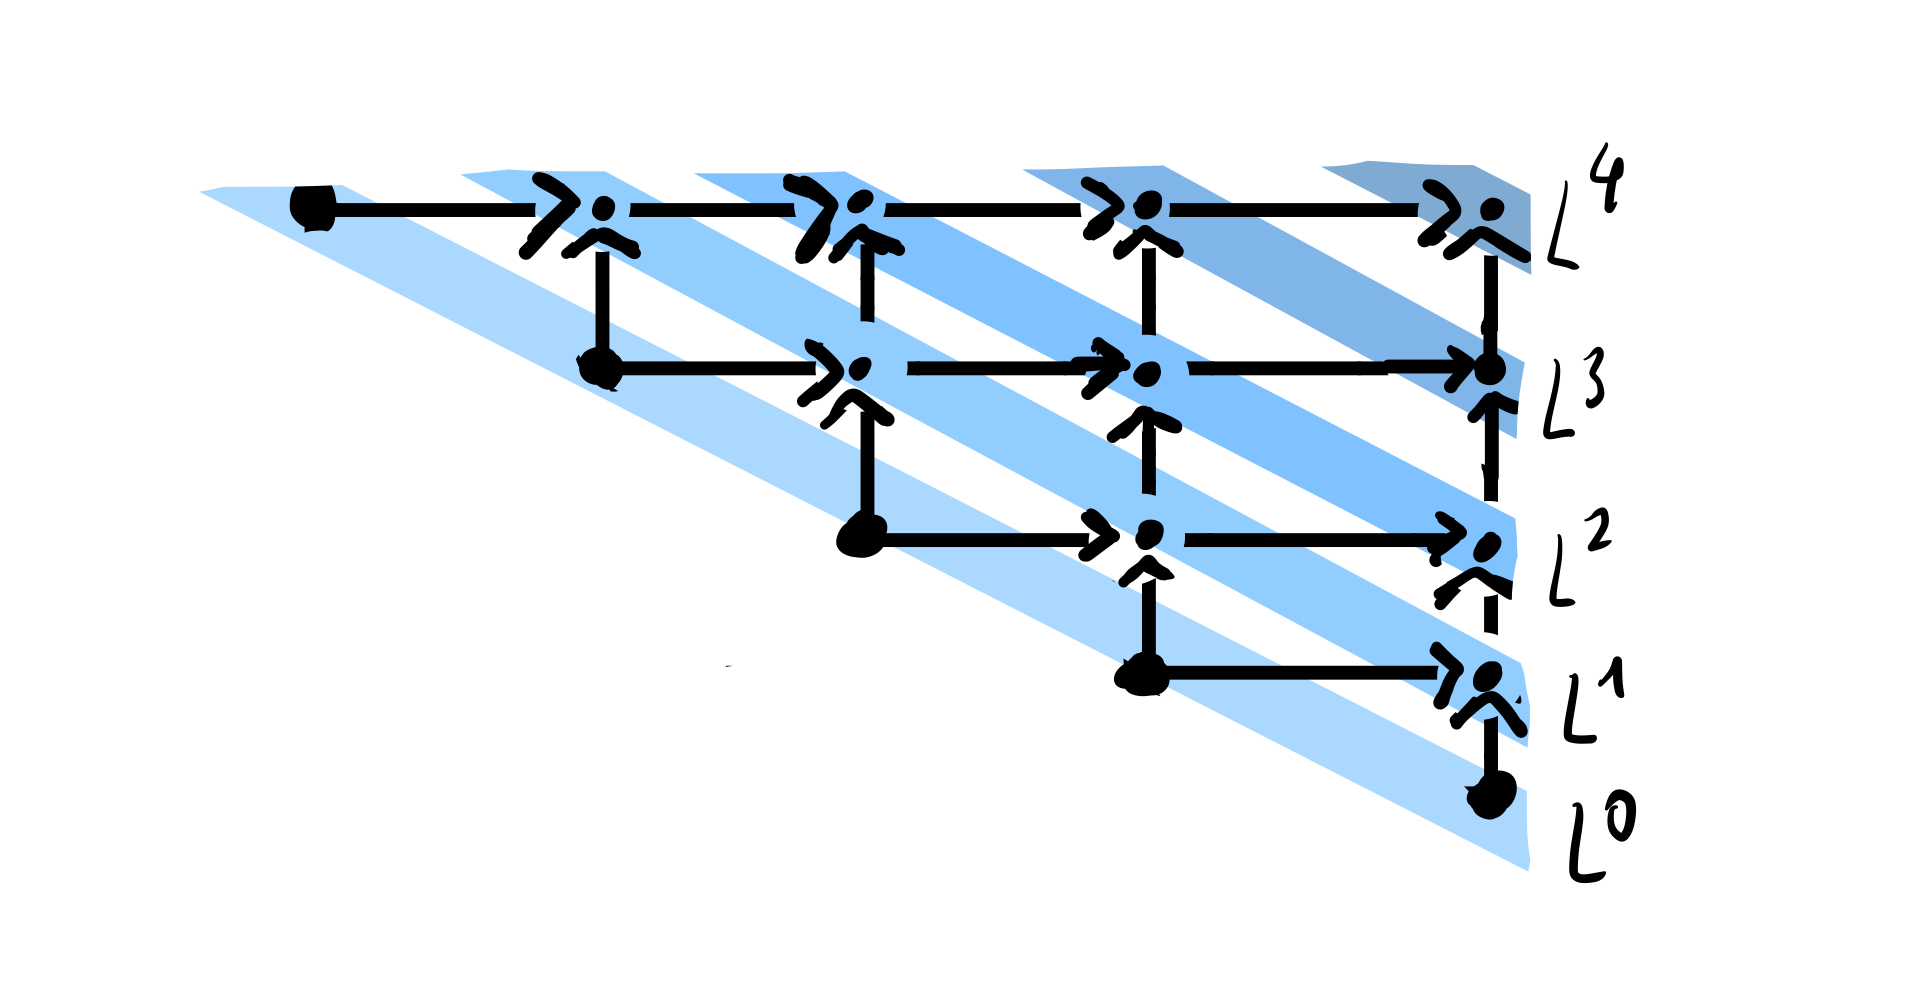
\includegraphics[width=0.6\textwidth,natwidth=1921,natheight=1000]{/Users/lapo_santi/Desktop/Nial/project/POMMs/level_sets.jpeg}
\caption{Visual Display of the level sets $L^k: k=0,\ldots,4$}
\label{fig:level_sets}
\end{center}
\end{figure}


The \textit{level sets} of $P$, in this case, corresponds to the diagonals above the main one.


\subsection{Partially ordered Markov Models applied to P}
\bigskip
Considering the finite set of random variables $\{P_{1,1},\dots, P_{K,K} \}$ indexed by locations where 
$$D\equiv \{(1,1), \dots (K,K)\}$$

Having showed the existence of a directly acyclic graph $ (P,F)$ and its corresponding poset $(P, \leq)$, we can write down 
\begin{align}
P(P_{ij}| Z(\text{cone } i,j)) &= P(P_{ij}| P(\text{adl } i,j))\\
P(P_{ij}| P_{i+1,j}, P_{i,j-1})
\end{align}

Now, exploiting Proposition \eqref{eq:result1}, we can write:
\begin{equation}
P(P(D)) = \prod_{i=1}^K\prod_{j=i}^K P(P_{ij}| P_{i+1,j}, P_{i,j-1})
\end{equation}


In order to induce an ordering or ranking among the blocks, we introduce a hierarchical structure. Without loss of generality, we assume that block 1 has the highest probability of success when interacting with any other block, while block $K$ has the lowest probability of success. We require this ranking to be transitive, meaning that if block A has a higher probability of success when interacting with block B, and block B has a higher probability of success when interacting with block C, then block A must still be the preferred choice when interacting with block C. Mathematically, this can be expressed as $p_{k,h} > p_{k',h}$ when $k < k'$ for $h \notin { k, k' }$.

To achieve this effect, we impose three conditions: probabilities should increase in the columns, decrease in the rows, and be greater than or equal to 0.5 in the upper triangular matrix. To satisfy these conditions, we construct the following scheme.

\subsubsection{Level Sets}

We define the level sets, denoted by $L^{(k)}$, as the diagonals of the upper triangular matrix P. The main diagonal is referred to as level set 0, denoted by $L^{(0)}$. The diagonal above it is denoted by $L^{(1)}$, and so on up to $L^{(K-1)}$. Each level set $L^{(k)}$ is formally defined as:

\begin{equation}
L^{(k)} := { p_{ij} \mid j-i = k } \quad \text{for } k = 0, \ldots, K-1
\end{equation}

It is worth noting that the cardinality of each level set is given by $|L^{(k)}| = K - k$ for $k = 0, \ldots, K-1$.

\subsubsection{Truncation Process}

Requiring that probabilities increase in the rows and decrease in the columns is equivalent to ensuring that the level sets satisfy the condition:

\begin{equation}
\max(L^{(k)}) < \min(L^{(k+1)}) \quad \text{for } k = 0, \ldots, K-1
\end{equation}

To enforce this behavior, we employ an increasing truncation process controlled by a parameter $\alpha$, with an upper bound given by $\beta_{\max}$.

We consider a generic power-law function $y = x^\alpha + 0.5$, which governs the rate of increase in the truncation process. Setting $f(0) = 0.5$ ensures that $L^{(0)}$ is greater than or equal to 0.5, satisfying the transitivity condition. The function $y$ is monotonically increasing for $x > 0$. To generate the truncations, we partition $y$ effectively by dividing the interval into $K$ equal-sized segments. The segment endpoints are computed as $x_k = \Delta \times k$ for $k = 0, \ldots, K$, where $\Delta = \left( \left(\beta_{\max} - 0.5\right)^{(1/\alpha)} - 0 \right) / K$. Mapping the cumulative sum of the segment endpoints back to $y$ yields $K$ truncation points denoted by $y^{(k)}$, which are defined as:

\begin{equation}
\label{eq:truncations}
y^{(k)} = \left( \frac{(\beta_{\max} - 0.5)^{(1/\alpha)}}{K} \times k \right)^\alpha + 0.5 \quad \text{for } k = 0, \ldots, K
\end{equation}

Notice that $f(0) = 0.5$ and $f(K) = \beta_{\max}$ by construction.

These truncation points provide the upper and lower bounds for the entries within the corresponding level sets, thereby ensuring the desired hierarchy and transitivity in the ranking.

Mathematically we have that:
\begin{equation}
y^{(k)} < p_ij \in L^{(k)} < y^{(k+1)}\quad  k = 0, \ldots, K-1 
\end{equation}

\subsubsection{The POMM Prior}

Finally, we put a prior on the matrix $P$ with this new structure in place.
We assume that entries $p_{ij} \in L^{(k)} \mid (y^{(k)} + y^{(k+1)}$ are identically and independently distributed according to a $\operatorname{Uniform}(y^{(k)},y^{(k+1)}$. We also put a log-normal hyper-prior on $\alpha$ such that 
\begin{equation}
\alpha \sim \operatorname{lognormal}(\mu_\alpha, \sigma^2_\alpha)
\end{equation}
where $\mu_\alpha, \sigma^2_\alpha$ are specified according to the normal parametrisation of the lognormal and are fixed to 1 and 2 respectively.
Altogether, the POMM prior on P is the following:
\begin{align}
p_{ij} \in L^{(k)} \mid y^{(k)},y^{(k+1)} &\sim (y^{(k)},y^{(k+1)} \\
\alpha &\sim \operatorname{Lognormal}\left(\mu_\alpha, \sigma^2_\alpha\right)
\end{align}
and where the truncations $y^{(k)}$ are derived as in \eqref{eq:truncations}.



\subsubsection{The POMM Prior 2}


Finally, we put a prior on the matrix $P$ with this new structure in place.
We assume that entries $p_{ij} \in L^{(k)} \mid (y^{(k)} + y^{(k+1)}$ are identically and independently distributed according to a $\operatorname{Normal}(\mu^{(k)},\sigma^{2(k)})$, where $\mu^{(k)} = \frac{y^{(k)}+y^{(k+1)}}{2}$ which corresponds to the midpoint of the level set $L^{(k)}$, and $\sigma^{2(k)} = \left( y^{(k)}+y^{(k+1)} \right) \times S$, where $S$ is a parameter denoted as \textit{overlap}, which intuitively is proportional to the overlap in the distribution support of the level sets.   We also put a log-normal hyper-prior on $\alpha$ such that 
\begin{equation}
\alpha \sim \operatorname{lognormal}(\mu_\alpha, \sigma^2_\alpha)
\end{equation}
where $\mu_\alpha, \sigma^2_\alpha$ are specified according to the normal parametrisation of the lognormal and are fixed to 1 and 2 respectively.
Altogether, the POMM prior on P is the following:
\begin{align}
p_{ij} \in L^{(k)} \mid y^{(k)},y^{(k+1)} &\sim \operatorname{Normal}\left(\mu^{(k)},\sigma^{2(k)}\right) \mathbb{I}(0.5, \beta_{\max}) \\
\alpha &\sim \operatorname{Lognormal}\left(\mu_\alpha, \sigma^2_\alpha\right)\\
S \sim &\sim \operatorname{Lognormal}\left(\mu_S, \sigma^2_S \right)
\end{align}
and where the truncations $y^{(k)}$ are derived as in \eqref{eq:truncations}.


Insert here the plot for 3 different overlap values





\begin{figure}[htbp]
    \centering
    \subfigure[$\alpha=1, S=0.2$]{%
        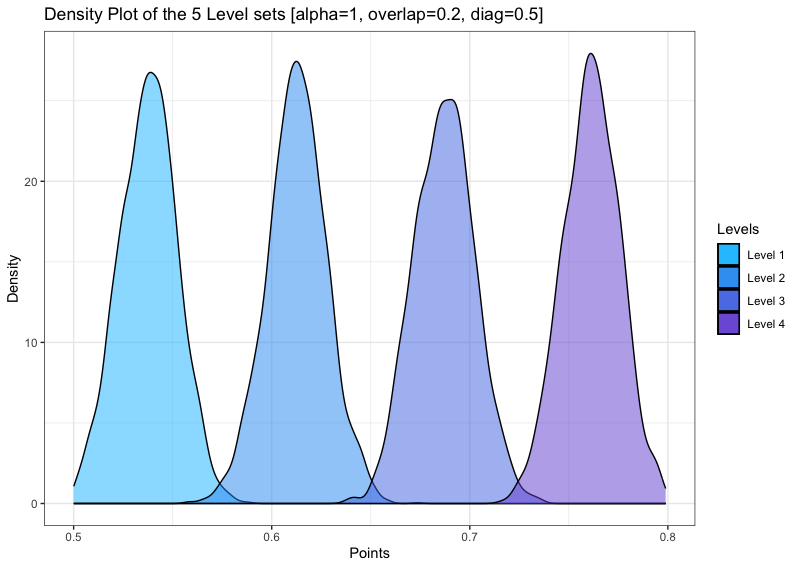
\includegraphics[width=.33\textwidth,natwidth=800,natheight=524]{/Users/lapo_santi/Desktop/Nial/POMM_pairwise/POMMs/POMM_flex/exploratory_graphs_with_inference/Densityplot_5_Level_sets_alpha__1__overlap__0.2__diag__0.5.png}%
        \label{fig:overlap0.2}%
    }\hfill
    \subfigure[$\alpha=1, S=0.5$]{%
        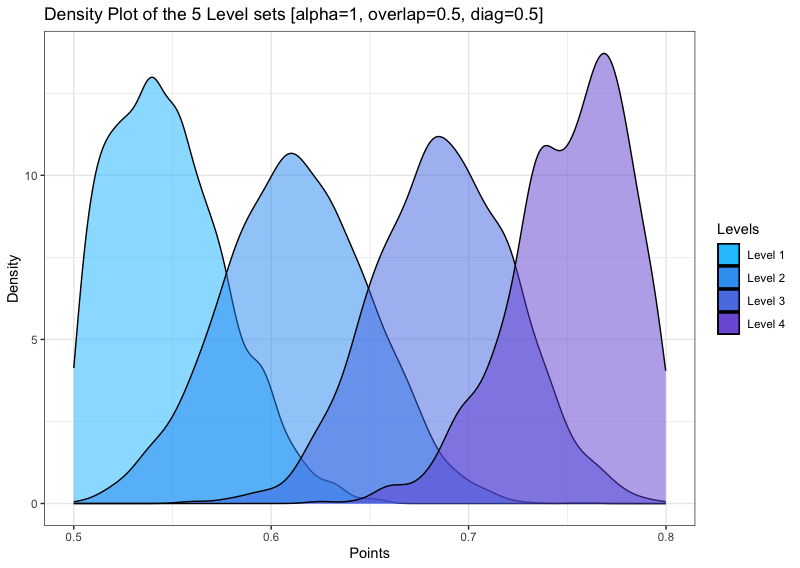
\includegraphics[width=.33\textwidth,natwidth=800,natheight=568]{/Users/lapo_santi/Desktop/Nial/POMM_pairwise/POMMs/POMM_flex/exploratory_graphs_with_inference/Densityplot_5_Level_sets_alpha__1__overlap__0.5__diag__0.5.png}%
        \label{fig:overlap0.5}%
    }\hfill
    \subfigure[$\alpha=1, S=0.8$]{%
        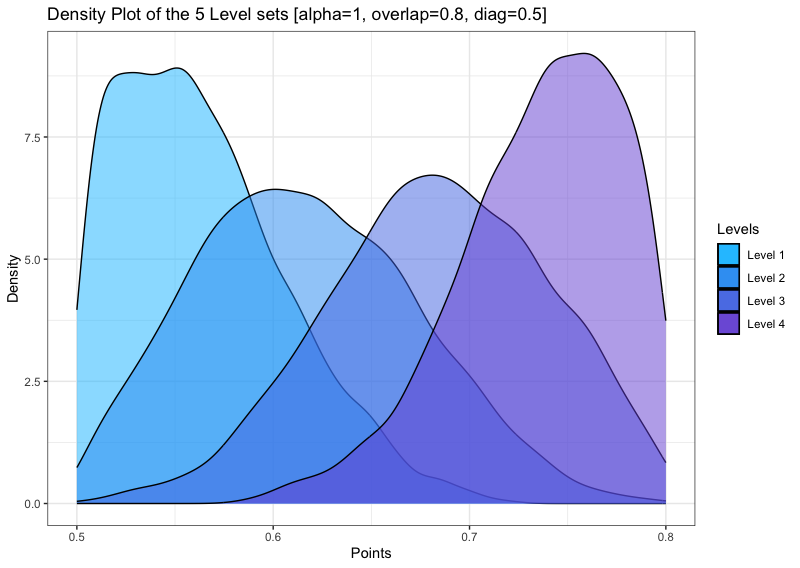
\includegraphics[width=.33\textwidth,natwidth=800,natheight=568]{/Users/lapo_santi/Desktop/Nial/POMM_pairwise/POMMs/POMM_flex/exploratory_graphs_with_inference/Densityplot_5_Level_sets_alpha__1__overlap__0.8__diag__0.5.png}%
        \label{fig:overlap0.8}%
    }
    \caption{Densities for $K=5$ Level Sets, for different $S$ values and $\alpha=1$; the main diagonal is set to 0.5, and its collapsed density is not reported.}
    \label{fig:all_images}
\end{figure} 

\subsection{Some notes on the overlap of two normal densities}


The computation or estimation of $S$, the overlap for two normal distributions, with density functions $\mathrm{f}_1\left(\mathrm{X} ; \mu_1, \sigma_1^2\right)$ and $\mathrm{f}_2\left(\mathrm{X} ; \mu_2, \sigma_2^2\right)$, depends on whether the two variances are equal. Since the estimation of OVL when $\sigma_1^2=\sigma_2^2=\sigma^2$ is simpler, has attracted more attention, and leads to firmer conclusions, we consider this situation in some detail. On the other hand, we shall simply summarise the results we have obtained in the more complicated circumstance when $\sigma_1^2 \neq \sigma_2^2$.

When $\sigma_1^2=\sigma_2^2$, the normal density functions intersect at the single value of $\mathrm{X}$ equal to $\left(\mu_1+\mu_2\right) / 2$. 

Representing the standard normal distribution function by $\Phi(\cdot)$, we obtain
$$
\mathrm{S}=2 \Phi\left(-\frac{\left|\mu_1-\mu_2\right|}{2 \sigma}\right)=2 \Phi\left(-\frac{1}{2}|\delta|\right)
$$

In our case we have that $\mu_1 < \mu_2 < \ldots < \mu_K$ and we are interested in the total overlap between the densities that are defined on the level sets. The total overlap is the sum of the pairwise overlaps between the densities taken two at a time:
\begin{align}
S &= \sum_{p=1}^{K-1} \sum_{q=i+1}^K S_{pq} \nonumber \\
&= \sum_{p=1}^{K-1} \sum_{q=i+1}^K  \Phi\left(-\frac{\left|\mu_p-\mu_q \right|}{2 \sigma}\right)\end{align}


Let's simplify the expression for the total overlap, denoted as S, using the fact that the means are ordered $\mu_1 < \mu_2 < \ldots < \mu_K$.

First, we can notice that for each pair of means $\mu_p$ and $\mu_q$, where $p < q$, we have the following relationship:
\begin{align*}
\mu_q - \mu_p &> 0 \quad \text{(since } \mu_1 < \mu_2 < \ldots < \mu_K \text{)} \\
\left|\mu_q - \mu_p \right| &= \mu_q - \mu_p \quad \text{(because it is positive)}
\end{align*}

Now, let's rewrite the total overlap S using this information:
\begin{align*}
S &= \sum_{p=1}^{K-1} \sum_{q=i+1}^K \Phi\left(-\frac{\left|\mu_p-\mu_q \right|}{2 \sigma}\right) \\
&= \sum_{p=1}^{K-1} \sum_{q=i+1}^K \Phi\left(-\frac{\mu_q - \mu_p}{2 \sigma}\right) \quad \text{(using the fact mentioned above)} \\
&= \sum_{p=1}^{K-1} \sum_{q=i+1}^K \Phi\left(-\frac{\mu_q}{2 \sigma} + \frac{\mu_p}{2 \sigma}\right) \\
\end{align*}







\clearpage
\section{Estimation}

For the moment, we want to infer just $\theta = \{ z, P, \alpha, S \}$, meaning that we treat $K$ as a known constant. The estimation strategy is a Hybrid MCMC algorithm. Since simulating from the conditional distribution $p(\theta_i| \theta_j, j\neq i)$ is unfeasible or computationally expensive, we substitute the simulation from the full conditional distribution with a simulation from a proposal distribution $q_i$. Referencing Muller's (1991) work, the Hybrid modification is as follows:

\begin{algorithm}
\begin{algorithmic}[h]
\For{$i = 1,\ldots, p \quad \texttt{given} \quad \left( \theta_1^{(t+1)}, \dots,\theta_{i-1}^{(t+1)},\theta_i^{(t)}, \dots,\theta_{p}^{(t)}\right)  $}
\State \texttt{1. Simulate} \begin{equation}\label{eqn_general_proposal}
\theta_i^{\prime} \sim q_i \left(\theta_i^{(t)} | \theta_1^{(t+1)}, \dots,\theta_{i}^{(t)},\theta_{i+1}^{(t)}, \dots,\theta_{p}^{(t)} \right)
\end{equation}
\State \texttt{2. Take} \begin{equation}\label{eqn_acc_reject}
\theta_i^{(t+1)} = 
\begin{cases}
\theta_{i}^{(t)} \quad &\texttt{with probability} \quad 1 - r_i, \\
\theta_{i}^{\prime} \quad &\texttt{with probability} \quad 1 - r_i,
\end{cases}
\end{equation}
\State \texttt{where} \begin{equation}\label{eqn_gen_ratio}
r_i = 1 \vertg \left\{
\frac{\left(p(\theta_i^{\prime}|\theta_i^{(t)} | \theta_1^{(t+1)}, \dots,\theta_{i}^{(t)},\theta_{i+1}^{(t)}, \dots,\theta_{p}^{(t)}\right)}{\left(p(\theta_i^{(t)}|\theta_i^{(t)} | \theta_1^{(t+1)}, \dots,\theta_{i}^{(t)},\theta_{i+1}^{(t)}, \dots,\theta_{p}^{(t)}\right)}\right\}
\end{equation}
\EndFor
\end{algorithmic}
\label{alg_general_algortm}
\caption{Metropolis-within-Gibbs MCMC}
\end{algorithm}


\subsubsection{Adaptive algorithm for $\theta = \{ P, \alpha, S \}$}

We specify the proposal distributions in \eqref{eqn_general_proposal} above as $$\theta_i^{\prime} \sim \operatorname{Normal}\left( \theta_i^{(t-1)}, \sigma_{\theta_i}^2 \right)$$ whose sampled value is accepted or rejected by evaluating the logarithm of \eqref{eqn_gen_ratio}. Choosing a correct $\sigma_{\theta_i}^2 $ value is not straightforward, and we choose to resort to an adaptive algorithm to elicitate a correct proposal variance. We proceed as in Roberts, Rosenthal 2012. For each of the $K(K-1)/2 + 2$ parameters \(i\) \((1 \leq i \leq K(K-1)/2 + 2)\), we create an associated variable \(ls_i\) giving the logarithm of the standard deviation to be used when proposing a normal increment to variable \(i\). We begin with \(ls_i = \log{(0.04)}\) for all \(i\) (corresponding to 0.2 proposal standard deviation). After the \(n\)-th "batch" of 50 iterations, we update each \(ls_i\) by adding or subtracting an adaption amount \(\delta(n)\). The adapting attempts to make the acceptance rate of proposals for variable \(i\) as close as possible to 0.234, following the literature practice Chris Sherlock12009. Specifically, we increase \(ls_i\) by \(\delta(n)\) if the fraction of acceptances of variable \(i\) was more than 0.234 on the \(n\)-th batch, or decrease \(ls_i\) by \(\delta(n)\) if it was less.

$\rightarrow$ Insert here plots of convergence to the acceptance ratio

We specify in the Appendix the full expression for the ratio of $\theta = \{ P, \alpha, S \}$ in \eqref{eqn_gen_ratio}.

\subsubsection{Adaptive Algorithm for $\theta = { z }$}

When dealing with $\theta = { z }$, a discrete parameter, we need to adapt the formulation while maintaining the underlying concept. In the case of the POMM model, the labels $k = 1, \ldots, K$ are ordered, and therefore, we can define a distance metric between these labels. Let us denote the distance between $k$ and $k'$ as $d(k, k')$, which can be expressed as:

\begin{equation}
d(k, k^\prime) = |k - k^\prime|
\end{equation}

If the acceptance rate for a particular player $i$ is too low, we want the proposal to explore neighboring labels. Conversely, if the acceptance rate is too high, we aim to sample labels further away. To achieve this, we assign a sampling probability to each label that is inversely related to its distance from the current label. Specifically, we define $p(k') = p(|k' - k|) = \operatorname{Normal}(0, \sigma_i^2)$, where $\sigma_i^2$ is adapted as above. A larger variance assigns higher probabilities to distant labels, while a smaller variance favors closer labels. Finally, we employ a multinomial distribution to sample the next label $k'$:

\begin{equation}
k' \sim \operatorname{Multinomial}(1, K, p(|k' - k|))
\end{equation}

By using this approach, we can adapt the algorithm to explore labels based on their distances from the current label. 

We specify in the Appendix the full expression for the ratio of $\theta = \{z\}$ in \eqref{eqn_gen_ratio}.




\clearpage

\section{Point Estimate, Model Selection,  and inference}

While algorithmic methods produce a single estimated partition, our model offers the entire posterior distribution across different node partitions. We are comparing the results from the simulation study via the following three main measures:

\begin{itemize}
\item Variation of Inforamation (VI): to fully utilise this posterior and engage in inference directly within the partition space, we adopt the decision-theoretic approach introduced by Wade and Ghahramani (2018) for block modeling. This involves summarizing posterior distributions using the variation of information (vi) metric, developed by Meilă (2007), which measures the distance between two clusterings by comparing their individual and joint entropies. The vi metric ranges from 0 to log2 V, where V represents the number of nodes. Intuitively, the vi metric quantifies the amount of information contained in two clusterings relative to the shared information between them. As a result, it decreases towards 0 as the overlap between two partitions increases. Refer to Wade and Ghahramani (2018) for a detailed exploration of the key properties of the vi metric. Within this framework, a formal Bayesian point estimate for z is obtained by selecting the partition with the lowest averaged vi distance from the other clusterings
\item WAIC: While the WAIC yields practical and theoretical advantages  and has direct connections with Bayesian leave-one-out cross-validation, thus providing a measure of edge predictive accuracy, the calculation of the WAIC only requires posterior samples of the log-likelihoods for the edges:$
\log p(y_{ij} | z, P, \alpha) = y_{ij} \log p_{z_i, z_j} + (n_{ij}- y_{ij}) \log(1 - p_{z_i, z_j}), \quad i = 2, \ldots, N,  j = 1, \ldots, i - 1$.

\item Misclassification error: predicting the group membership $z_{N+1}$ of a new player may also be of interest. We can derive the estimate of the block probabilities for new players based on their early matches with some of the existing players.
\begin{align}
p(z_{N+1} = k | \textbf{Y}, y_{N+1}, \hat{z}) &\propto p(y_{N+1} | \textbf{Y}, \hat{z}, z_{N+1} = k ) \cdot p(z_{N+1} = k | \hat{z}) \nonumber \\
&= p(y_{N+1} | \hat{z}, z_{N+1} = k ) \cdot p(z_{N+1} = k | \hat{z})
\end{align}
where $p(z_{N+1} = k | \textbf{Y}, y_{N+1}, \hat{z})$ is the posterior probability of the new node $N+1$ to belong to the block $k$, given the previously observed data $Y$, the new node's data $y_{N+1}$ and the estimated labels $\hat{z}$. On the right hand side of the expression above, $p(y_{N+1} | \textbf{Y}, \hat{z}, z_{N+1} = k )$ represents the likelihood of observing $y_{N+1}$ given the previously observed data $Y$ and the estimated labels $\hat{z}$, which, due to conditional independence, is the same as conditioning just on $\hat{z}$. Finally, $p(z_{N+1} = k | \hat{z})$ represents the prior probability of label $k$ for the new node $N+1$ given $\hat{z}$, which we can approximate with the relative size of the blocks $n_k$.
\end{itemize}
\begin{comment}
\item Prediction error: making prediction on the match score between two players is also possible within this framework. Once we have obtained the MCMC samples, we can retrieve the posterior predictive distribution.

Let us assume $i^\star$ is a new player . The posterior predictive is:
\begin{align}
p(y_{i^\star j}| \textbf{Y}) &= \int p(z| \{ \textbf{Y}\setminus y_{i^\star} \})  \cdot p(y_{i^\star j} | z ) dz \\
&\approx \frac{1}{T} \sum_{t = 1}^{T} \sum_{z_i=1}^{K}  p(y_{i^\star j}| z_j^{(t)}) \\
&=  \frac{1}{T} \sum_{t = 1}^{T} \sum_{z_{i^\star} =1}^{K}  p_{z_{i^\star}, z_j^{(t)}}^{y_{i^\star j} } \cdot (1-p_{z_{i^\star}, z_j^{(t)}})^{n_{i^\star j} -  y_{i^\star j}} \quad \quad \text{for }y_{i^\star j} = 0,\ldots, n_{i^\star j} \\
\end{align} 
where $z_j^{(t)} \sim p(z|Y)$
\end{itemize}
\end{comment}

\clearpage

\section{Simulation Study from the Simple Model N=100}

In order to evaluate how well our model performs in a situation similar to our intended use, and measure its advantages compared to the best existing alternatives, we generated three simulated tournaments with 100 players from the Simple Model. We want to compare how it performs compared to the POMM extension and other state-of-the-art alternatives. Each tournament had a different number of blocks in the underlying structure. We set the total number of games $M := 0.5* \sum_{i,j}^N n_{ij}= \sum_{i,j}^N y_{ij} = 4000$, which is the average number of matches played in one year of tennis tournaments. We divided the players into three, five and nine blocks ($K = 3,5,9$ respectively). In Figure (\ref{fig:simple_adjacency}), we display the three simulated tournaments, where the difficulty of accurately determining the group membership increases as the number of games increases with the number of blocks.

\begin{figure}[htbp]
    \centering
    \subfigure[K=3, Simple Model]{%
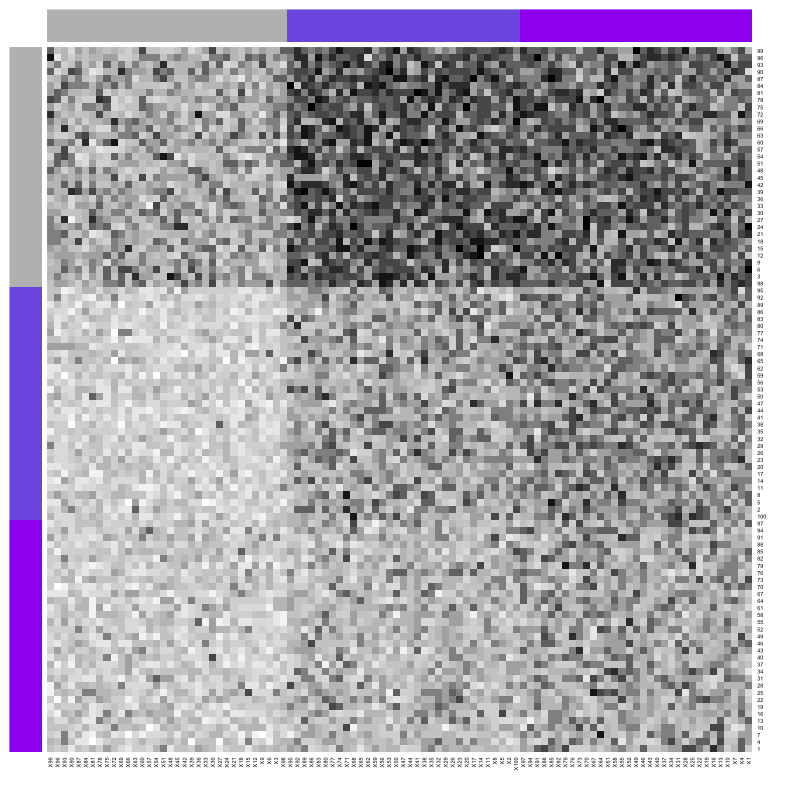
\includegraphics[width=.33\textwidth,natwidth=800,natheight=800]{  /Users/lapo_santi/Desktop/Nial/POMM_pairwise/POMMs/POMM_flex/MCMC/results_29_07/tables_and_plots/plots/adjacency_True_ModelSimpleEst_model_Simple_K3_N100.png}%
        \label{fig:simple_adjacency_K3}%
    }\hfill
    \subfigure[K=5, Simple Model]{%
        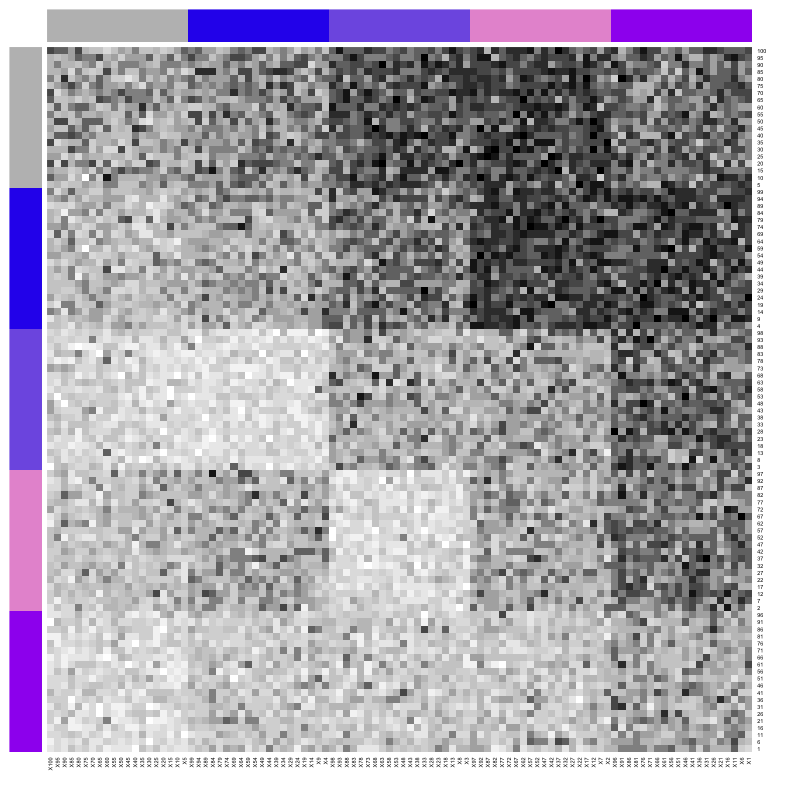
\includegraphics[width=.33\textwidth,natwidth=800,natheight=800]{  /Users/lapo_santi/Desktop/Nial/POMM_pairwise/POMMs/POMM_flex/MCMC/results_29_07/tables_and_plots/plots/adjacency_True_ModelSimpleEst_model_Simple_K5_N100.png}%
        \label{fig:simple_adjacency_K5}%
    }\hfill
    \subfigure[K=9, Simple Model]{%
        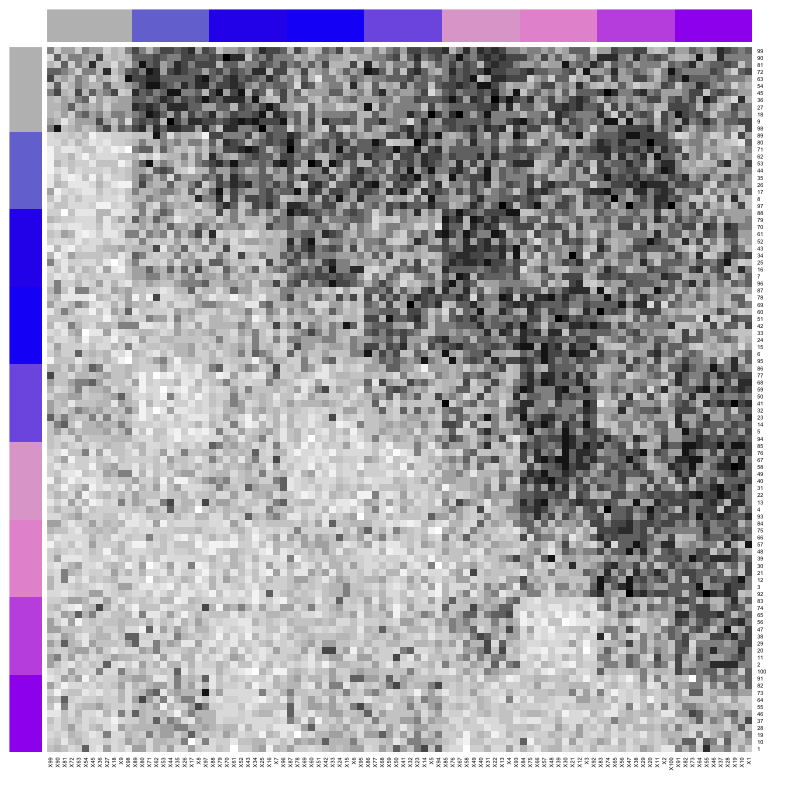
\includegraphics[width=.33\textwidth,natwidth=800,natheight=800]{  /Users/lapo_santi/Desktop/Nial/POMM_pairwise/POMMs/POMM_flex/MCMC/results_29_07/tables_and_plots/plots/adjacency_True_ModelSimpleEst_model_Simple_K9_N100.png}%
        \label{fig:simple_adjacency_K9}%
    }
    \caption{Adjacency Matrices simulated via the Simple Model}
    \label{fig:simple_adjacency}
\end{figure}

We compare the performance of the Simple model with the POMM one. We fixed arbitrarily $\beta_{\max} = .75$.
In table (\ref{table:simulations_from_simple}) we report the results of the simulation. In the three cases, for the Simple and the POMM model, we compare the WAIC, the VI distance and the misclassification error, obtained by considering 100 new incoming players which get to play just with 10 players each. We also compare the labels estimated against the regularised spectral clustering algorithm and the Louvain algorithm. The Simple model is the best performing relative to the other three alternatives.

\begin{figure}[htbp]
    \centering
    \subfigure[K=3, Simple Model]{%
        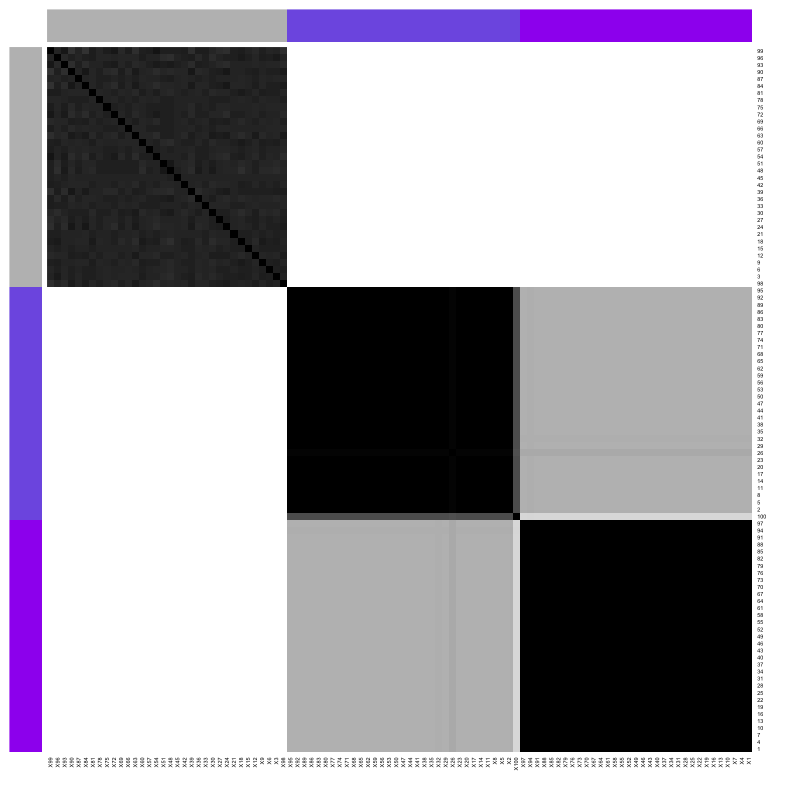
\includegraphics[width=.3333\textwidth,natwidth=800,natheight=800]{  /Users/lapo_santi/Desktop/Nial/POMM_pairwise/POMMs/POMM_flex/MCMC/results_29_07/tables_and_plots/plots/similarity_True_ModelSimpleEst_model_Simple_K3_N100.png}%
        \label{fig:M4000}%
    }\hfill
    \subfigure[K=5, Simple Model]{%
        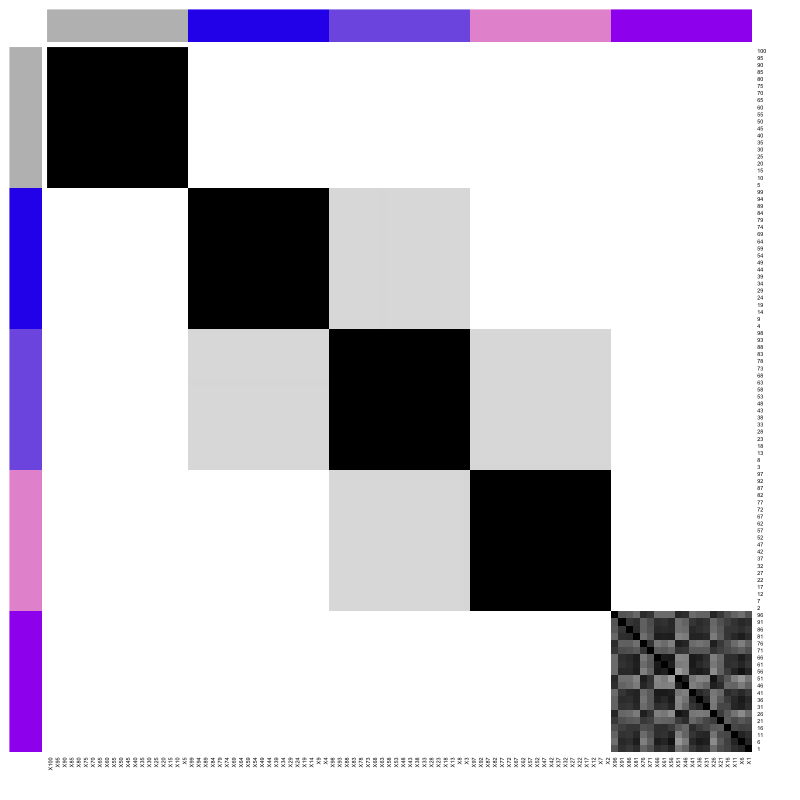
\includegraphics[width=.3333\textwidth,natwidth=800,natheight=800]{  /Users/lapo_santi/Desktop/Nial/POMM_pairwise/POMMs/POMM_flex/MCMC/results_29_07/tables_and_plots/plots/similarity_True_ModelSimpleEst_model_Simple_K5_N100.png}%
        \label{fig:M7000}%
    }\hfill
    \subfigure[K=9, Simple Model]{%
        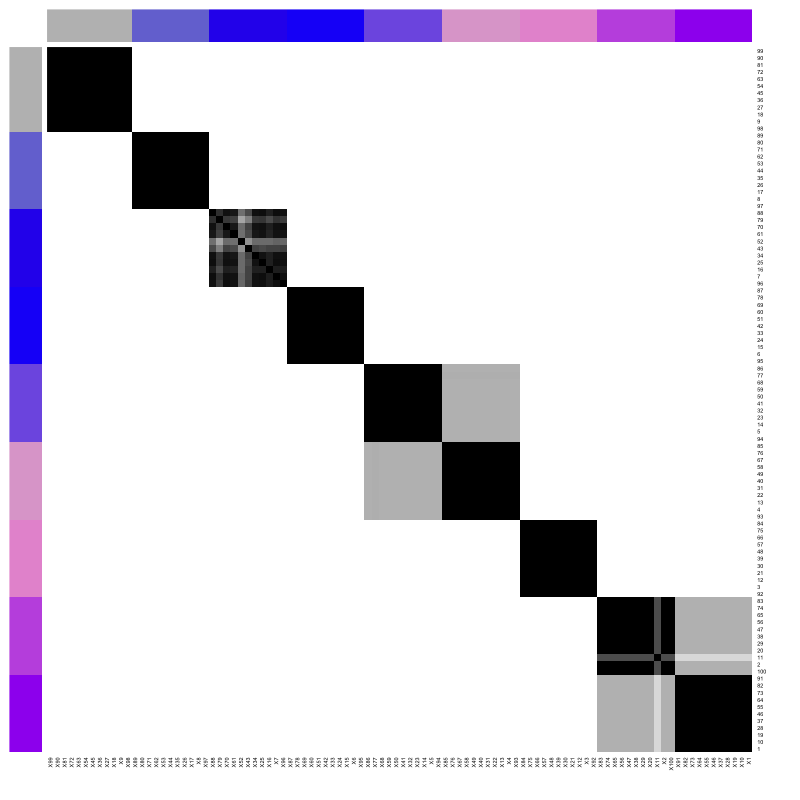
\includegraphics[width=.3333\textwidth,natwidth=800,natheight=800]{  /Users/lapo_santi/Desktop/Nial/POMM_pairwise/POMMs/POMM_flex/MCMC/results_29_07/tables_and_plots/plots/similarity_True_ModelSimpleEst_model_Simple_K9_N100.png}%
        \label{fig:M10000}%
    }\\[2ex]\subfigure[K=3, POMM Model]{%
        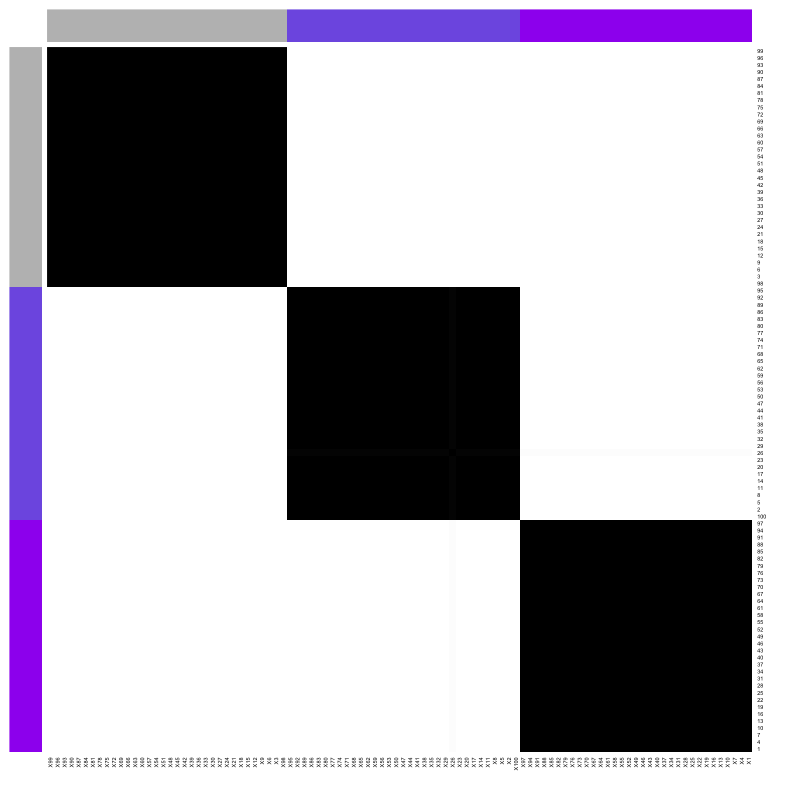
\includegraphics[width=.3333\textwidth,natwidth=800,natheight=800]{  /Users/lapo_santi/Desktop/Nial/POMM_pairwise/POMMs/POMM_flex/MCMC/results_29_07/tables_and_plots/plots/similarity_True_ModelSimpleEst_model_POMM_K3_N100.png}%
        \label{fig:M4000}%
    }\hfill
    \subfigure[K=5, POMM Model]{%
        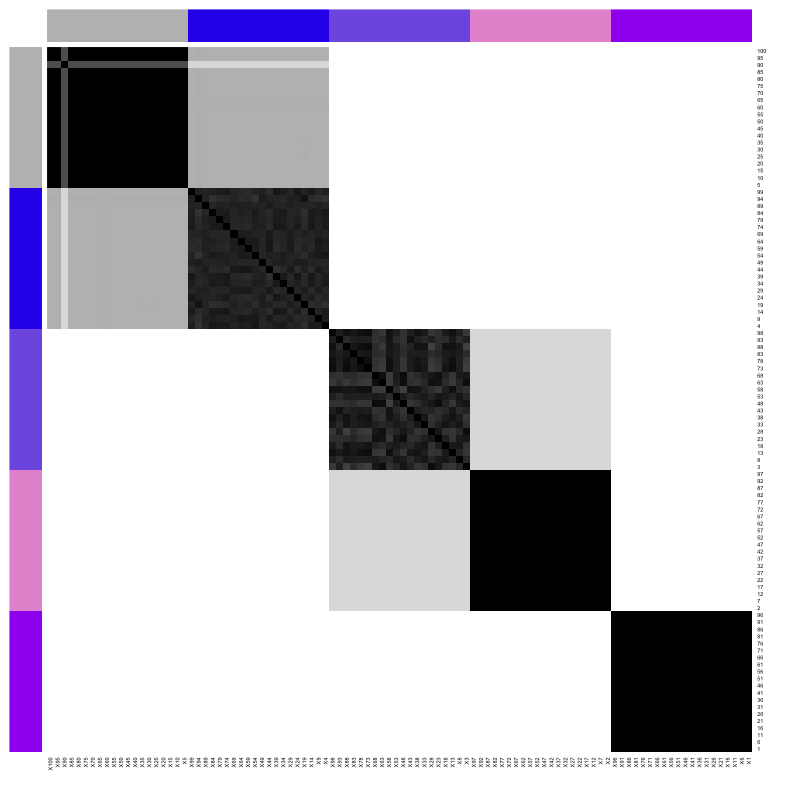
\includegraphics[width=.3333\textwidth,natwidth=800,natheight=800]{  /Users/lapo_santi/Desktop/Nial/POMM_pairwise/POMMs/POMM_flex/MCMC/results_29_07/tables_and_plots/plots/similarity_True_ModelSimpleEst_model_POMM_K5_N100.png}%
        \label{fig:M7000}%
    }\hfill
    \subfigure[K=9, POMM Model]{%
        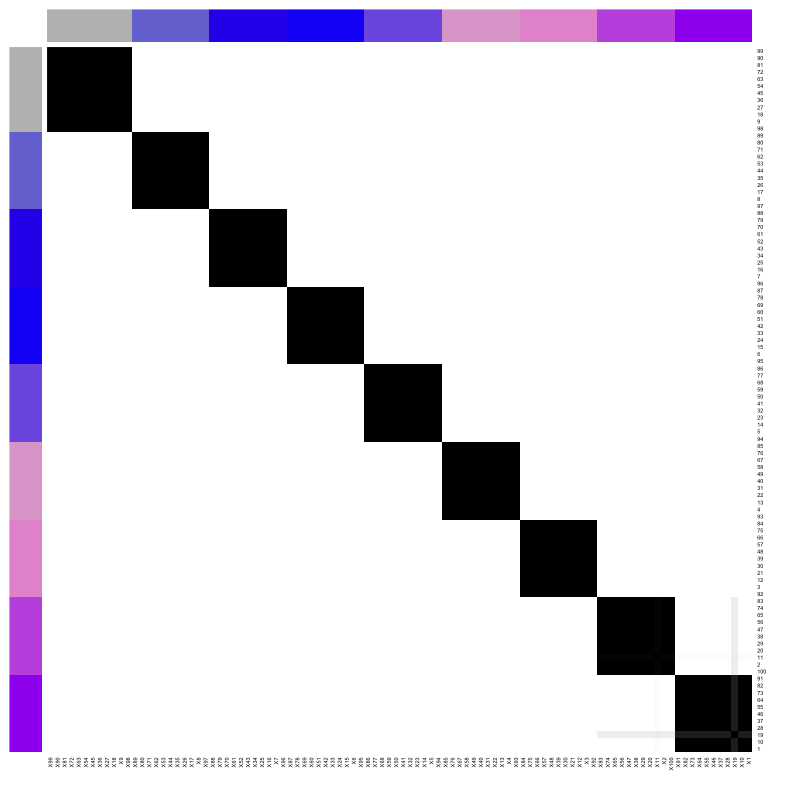
\includegraphics[width=.3333\textwidth,natwidth=800,natheight=800]{  /Users/lapo_santi/Desktop/Nial/POMM_pairwise/POMMs/POMM_flex/MCMC/results_29_07/tables_and_plots/plots/similarity_True_ModelSimpleEst_model_POMM_K9_N100.png}%
        \label{fig:M10000}%
    }
    \caption{Co-Clustering Matrices obtained via the Simple Model(above) and the POMM model (below).}
    \label{fig:adjacency_all_simple}
\end{figure}


In figure (\ref{fig:adjacency_all_simple}) we report the estimated co-clustering matrices resulting from the simulation process.


\begin{table}[htbp]
\centering
\caption*{
{\large $P$ summary table} \\ 
{\small True Model Simple, $N=100$}
} 
\begin{tabular}{cccccccccc}
\toprule
\multirow{2}{*}{Fitted Model} & \multicolumn{3}{c}{
$\overline{MAE}$ } & \multicolumn{3}{c}{
$\%$ within-95\% CI interval} & \multicolumn{3}{c}{ $\overline{\text{CI interval length}}$} \\
\cmidrule(lr){2-4} \cmidrule(lr){5-7} \cmidrule(lr){8-10}
& $(a)$ & $(b)$ & $(c)$ & $(a)$ & $(b)$ & $(c)$ & $(a)$ & $(b)$ & $(c)$ \\
\midrule
POMM model  &0.0602&  0.0179 & 0.0170 & 100$\%$  & 100$\%$   & 100$\%$  & 0.1344 & 0.1309 & 0.0837  \\
Simple model & 0.0601 &  0.0274 & 0.0140 & 100$\%$ &100$\%$  & 100$\%$  & 0.1344 & 0.1311 & 0.0871 \\
\bottomrule
\end{tabular}
\label{table:simulations_from_simple}
\end{table}


\begin{table}[htbp]
\centering
\caption*{
{\large $z$ summary table} \\ 
{\small True Model Simple, $N=100$}
} 
\begin{tabular}{cccccccccc}
\toprule
\multirow{2}{*}{Method} & \multicolumn{3}{c}{
VI $\text{distance}_{\text{MAP}}$} & \multicolumn{3}{c}{
VI $\text{distance}_{\text{VI lb}}$} & \multicolumn{3}{c}{WAIC} \\
\cmidrule(lr){2-4} \cmidrule(lr){5-7} \cmidrule(lr){8-10}
& $(a)$ & $(b)$ & $(c)$ & $(a)$ & $(b)$ & $(c)$ & $(a)$ & $(b)$ & $(c)$ \\
\midrule
POMM model  &0.22&  0 & 0.1 & 0.66 & 0  & 0.1 & $\underset{17.60}{-6481.92}$ & $\underset{17.76}{-6573.49}$ & $\underset{17.95}{6662.23}$  \\
Simple model & 0.22 &  0 & 0.09 & 0.66&0 &0.09 & $\underset{17.60}{6481.87}$ & $\underset{17.84}{6596.61}$ & $\underset{17.96}{6663.48}$ \\
\bottomrule
\end{tabular}
\label{table:simulations_from_simple}
\end{table}




\clearpage






\section{Simulation Study from the POMM Model N=100}

In this section we reverse the exercise performed in previous one. Before we were simulating from the Simple model, now we are doing the same, with similar parameters ($K=3,5,9, M=4000 \text{ and } \beta_{\max} = .75)$. Here are the results.

\begin{figure}[h]
    \centering
    \subfigure[K=3, POMM Model]{%
        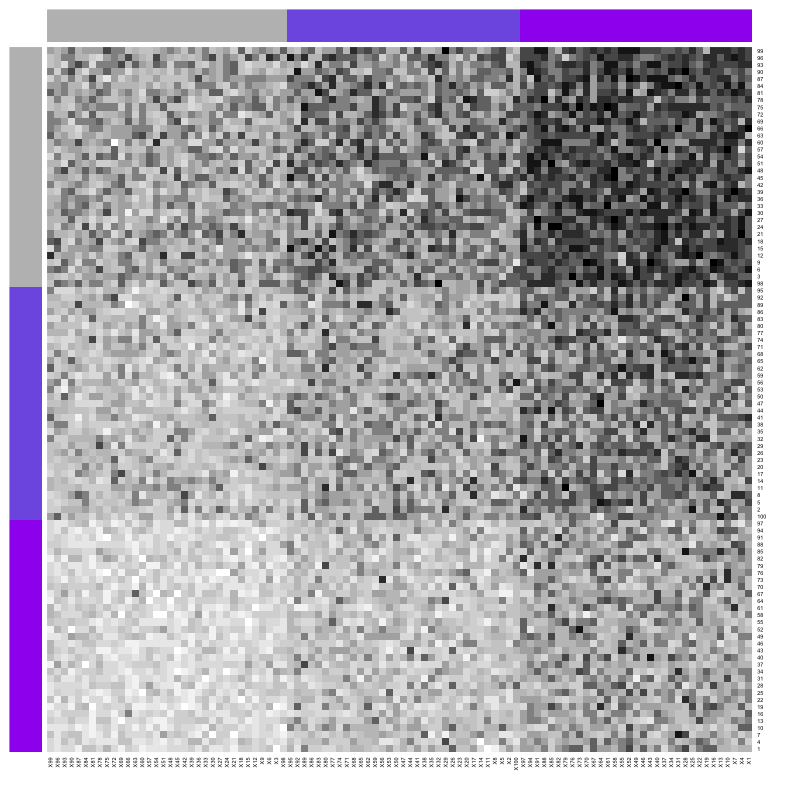
\includegraphics[width=.33\textwidth,natwidth=800,natheight=800]{  /Users/lapo_santi/Desktop/Nial/POMM_pairwise/POMMs/POMM_flex/MCMC/results_29_07/tables_and_plots/plots/adjacency_True_ModelPOMMEst_model_POMM_K3_N100.png}%
        \label{fig:POMM_adjacency_K3}%
    }\hfill
    \subfigure[K=5, POMM Model]{%
        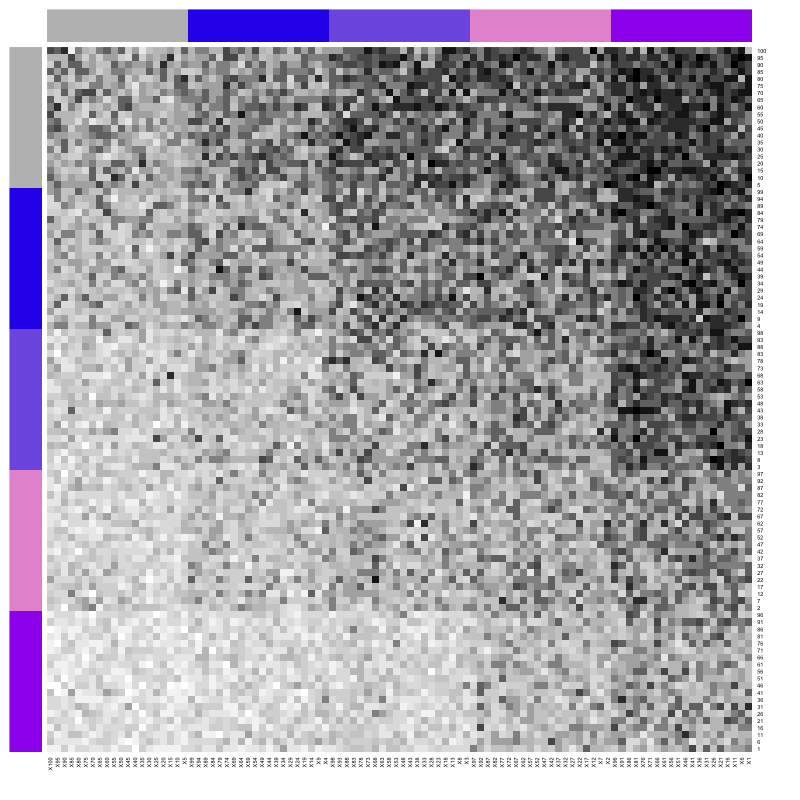
\includegraphics[width=.33\textwidth,natwidth=800,natheight=800]{/Users/lapo_santi/Desktop/Nial/POMM_pairwise/POMMs/POMM_flex/MCMC/results_29_07/tables_and_plots/plots/adjacency_True_ModelPOMMEst_model_POMM_K5_N100.png}%
        \label{fig:POMM_adjacency_K5}%
    }\hfill
    \subfigure[K=9, POMM Model]{%
        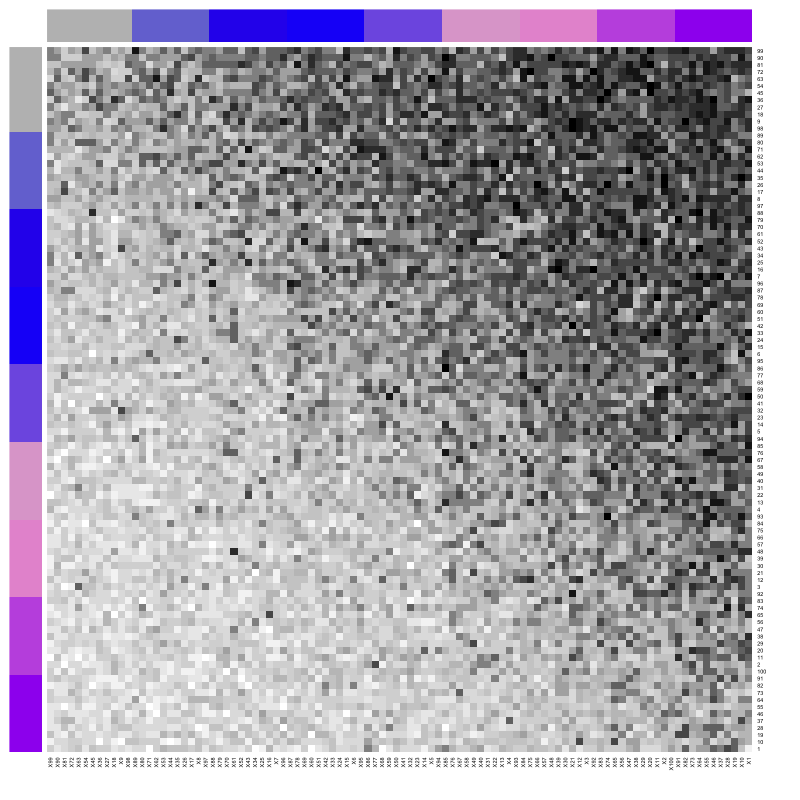
\includegraphics[width=.33\textwidth,natwidth=800,natheight=800]{ /Users/lapo_santi/Desktop/Nial/POMM_pairwise/POMMs/POMM_flex/MCMC/results_29_07/tables_and_plots/plots/adjacency_True_ModelPOMMEst_model_POMM_K9_N100.png}%
        \label{fig:POMM_adjacency_K9}%
    }
    \caption{Adjacency Matrices simulated via the POMM Model}
    \label{fig:all_images}
\end{figure}

\begin{figure}[htbp]
    \centering
    \subfigure[K=3, Simple Model Estimates]{%
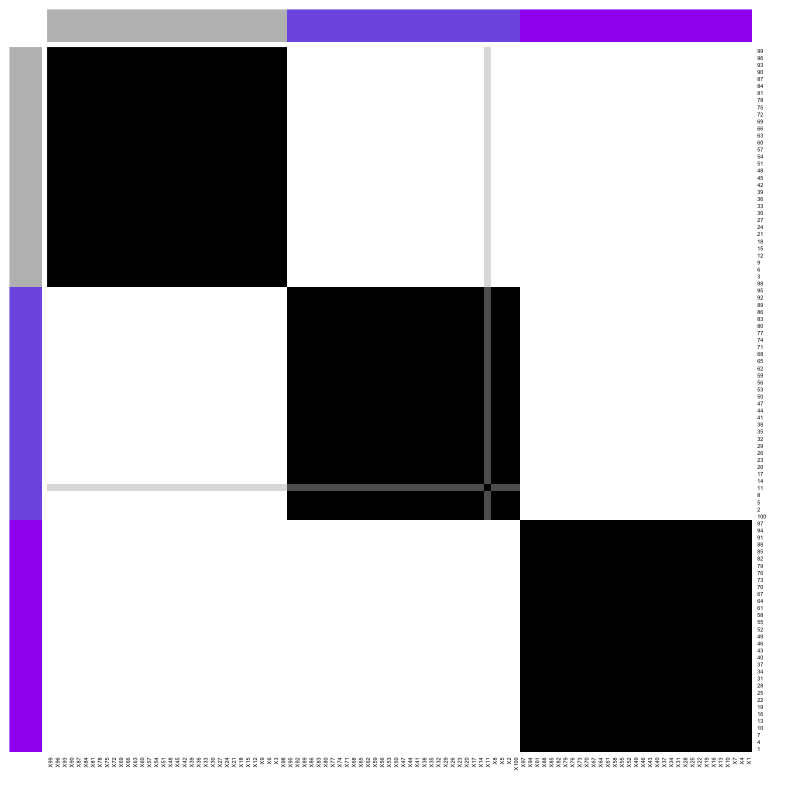
\includegraphics[width=.3333\textwidth,natwidth=800,natheight=800]{ /Users/lapo_santi/Desktop/Nial/POMM_pairwise/POMMs/POMM_flex/MCMC/results_29_07/tables_and_plots/plots/similarity_True_ModelPOMMEst_model_Simple_K3_N100.png}%
        \label{fig:M4000}%
    }\hfill
    \subfigure[K=5, Simple Model Estimates]{%
        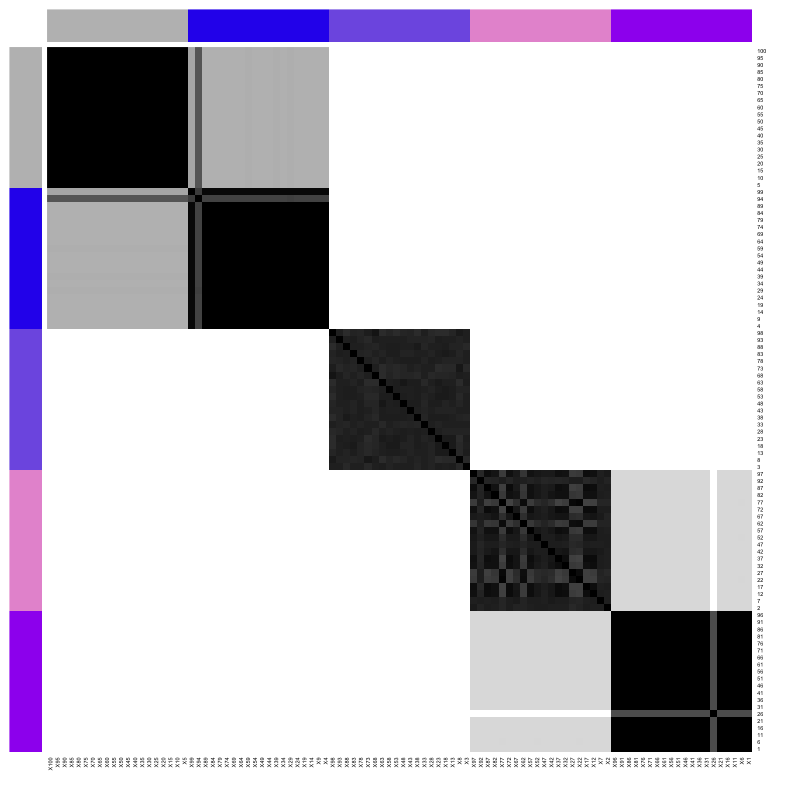
\includegraphics[width=.3333\textwidth,natwidth=800,natheight=800]{ /Users/lapo_santi/Desktop/Nial/POMM_pairwise/POMMs/POMM_flex/MCMC/results_29_07/tables_and_plots/plots/similarity_True_ModelPOMMEst_model_Simple_K5_N100.png}%
        \label{fig:M7000}%
    }\hfill
    \subfigure[K=9, Simple Model Estimates]{%
        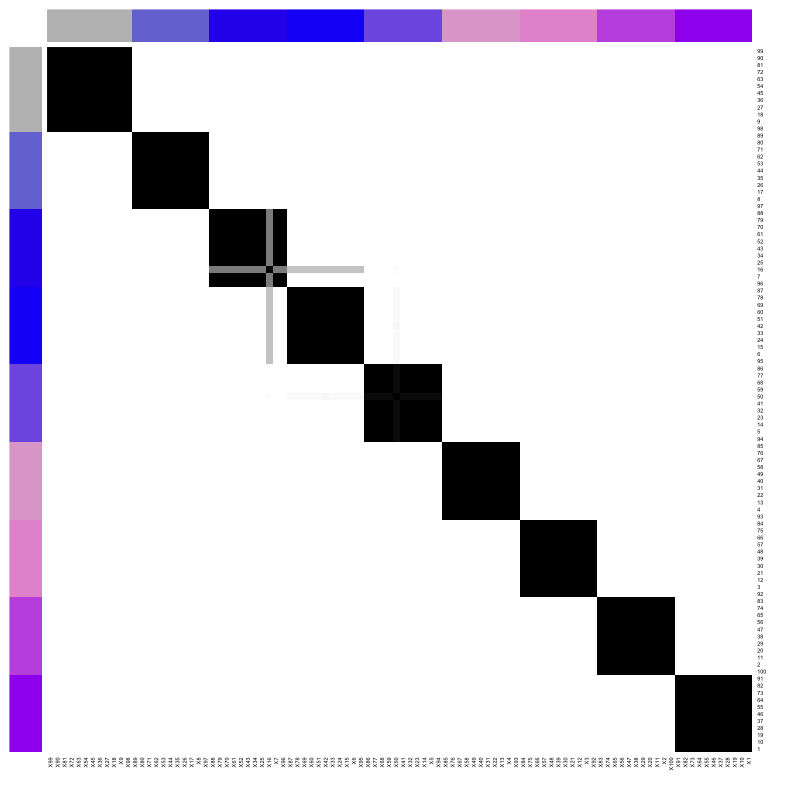
\includegraphics[width=.3333\textwidth,natwidth=800,natheight=800]{ /Users/lapo_santi/Desktop/Nial/POMM_pairwise/POMMs/POMM_flex/MCMC/results_29_07/tables_and_plots/plots/similarity_True_ModelPOMMEst_model_Simple_K9_N100.png}%
        \label{fig:M10000}%
    }\\[2ex]\subfigure[K=3, POMM Model Estimates]{%
        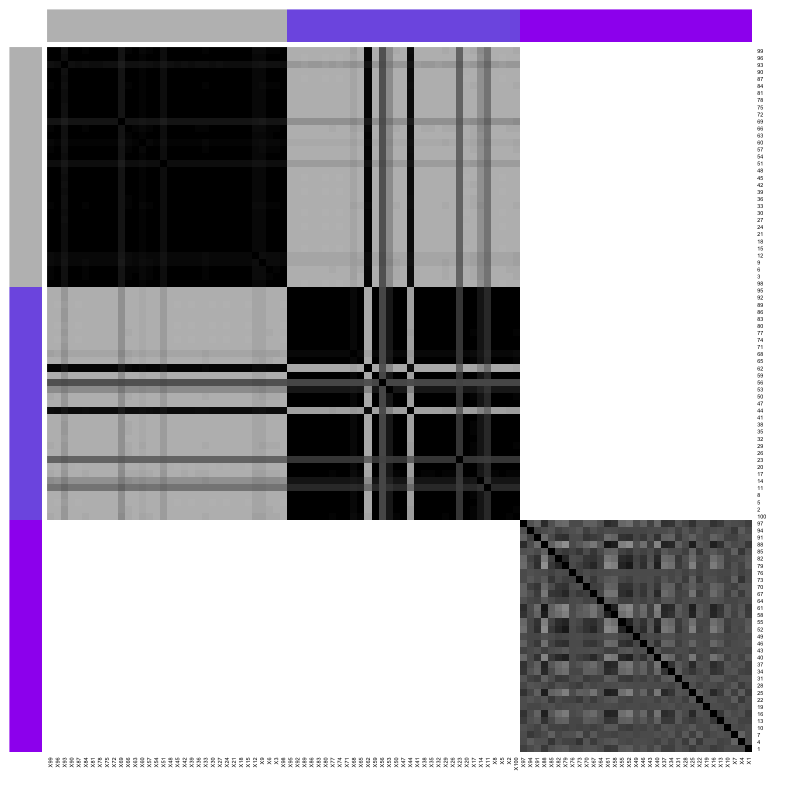
\includegraphics[width=.3333\textwidth,natwidth=800,natheight=800]{ /Users/lapo_santi/Desktop/Nial/POMM_pairwise/POMMs/POMM_flex/MCMC/results_29_07/tables_and_plots/plots/similarity_True_ModelPOMMEst_model_POMM_K3_N100.png}%
        \label{fig:M4000}%
    }\hfill
    \subfigure[K=5, POMM Model Estimates]{%
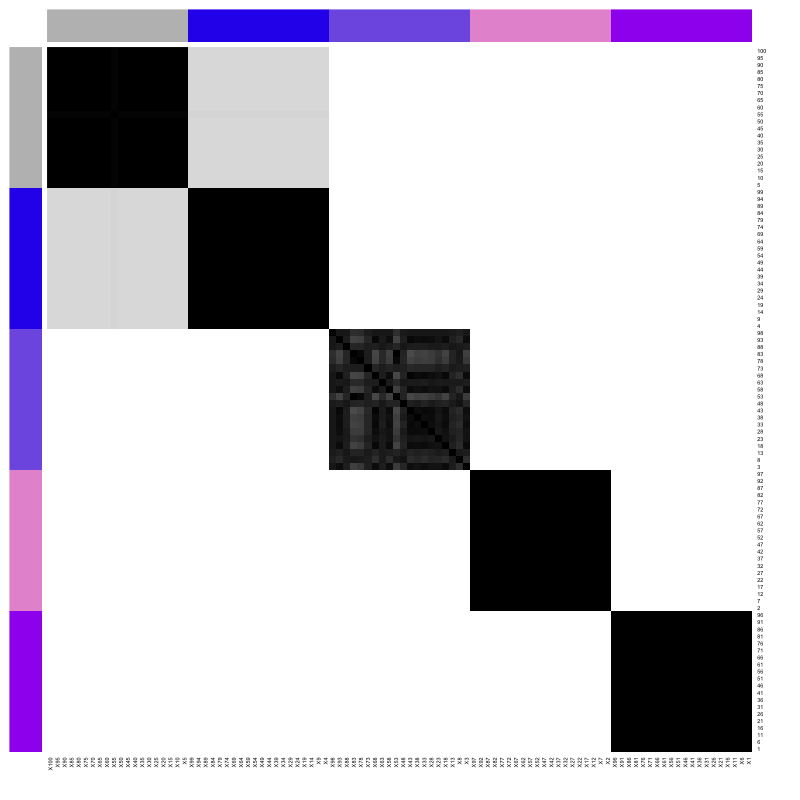
\includegraphics[width=.3333\textwidth,natwidth=800,natheight=800]{ /Users/lapo_santi/Desktop/Nial/POMM_pairwise/POMMs/POMM_flex/MCMC/results_29_07/tables_and_plots/plots/similarity_True_ModelPOMMEst_model_POMM_K5_N100.png}%
        \label{fig:M7000}%
    }\hfill
    \subfigure[K=9, POMM Model Estimates]{%
        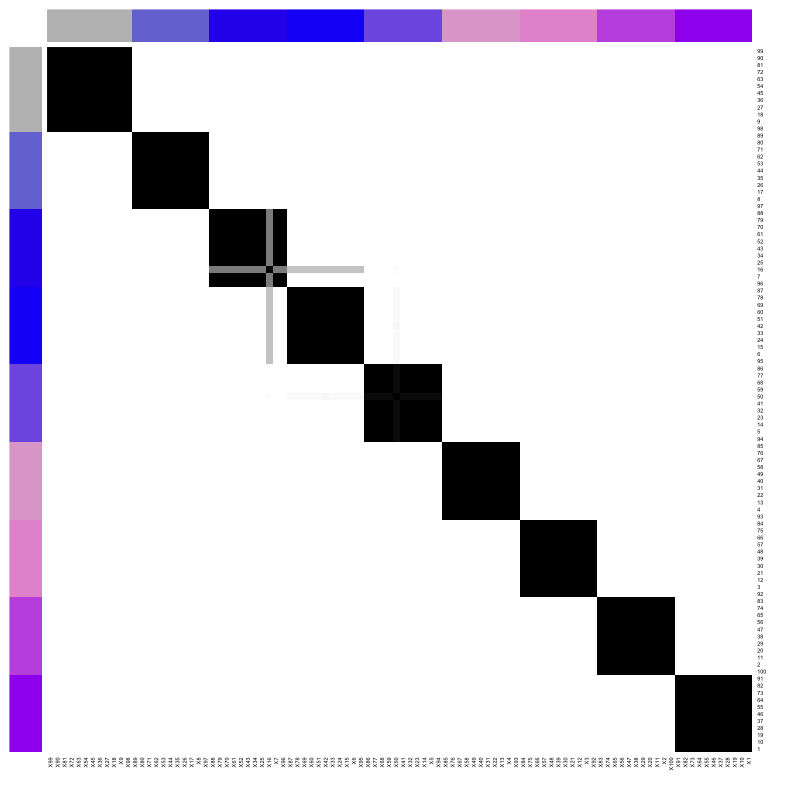
\includegraphics[width=.3333\textwidth,natwidth=800,natheight=800]{ /Users/lapo_santi/Desktop/Nial/POMM_pairwise/POMMs/POMM_flex/MCMC/results_29_07/tables_and_plots/plots/similarity_True_ModelPOMMEst_model_Simple_K9_N100.png}%
        \label{fig:M10000}%
    }
    \caption{Co-Clustering Matrices obtained via the Simple Model(above) and the POMM model (below).}
    \label{fig:all_images}
\end{figure}



In table (\ref{table:simulations_from_simple}) we report the results of the simulation. As before, for the Simple and the POMM model, we compare the WAIC, the VI distance and the misclassification error, obtained $N_new = 100$. Also here we compare clustering performance against that of the regularised spectral clustering algorithm and the Louvain algorithm. The POMM model is the best performing relative to the other three alternatives.

\begin{table}[htbp]
\centering
\caption*{
{\large $P$ summary table} \\ 
{\small True Model POMM, $K=3$, $N=100$}
} 
\begin{tabular}{cccccccccc}
\toprule
\multirow{2}{*}{Fitted Model} & \multicolumn{3}{c}{
$\overline{MAE}$ } & \multicolumn{3}{c}{
$\%$ within-95\%-CI interval} & \multicolumn{3}{c}{ $\overline{\text{CI interval length}}$} \\
\cmidrule(lr){2-4} \cmidrule(lr){5-7} \cmidrule(lr){8-10}
& $(a)$ & $(b)$ & $(c)$ & $(a)$ & $(b)$ & $(c)$ & $(a)$ & $(b)$ & $(c)$ \\
\midrule
POMM model  &0.0602&  0.0179 & 0.0170 & 100$\%$  & 100$\%$   & 100$\%$  & 0.1344 & 0.1309 & 0.0837  \\
Simple model & 0.0601 &  0.0274 & 0.0140 & 100$\%$ &100$\%$  & 100$\%$  & 0.1344 & 0.1311 & 0.0871 \\
\bottomrule
\end{tabular}
\label{table:simulations_from_simple}
\end{table}


\begin{table}[htbp]
\centering
\caption*{
{\large $z$ summary table} \\ 
{\small True Model POMM, $N=100$}
} 
\begin{tabular}{cccccccccc}
\toprule
\multirow{2}{*}{Method} & \multicolumn{3}{c}{
VI $\text{distance}_{\text{MAP}}$} & \multicolumn{3}{c}{
VI $\text{distance}_{\text{VI lb}}$} & \multicolumn{3}{c}{WAIC} \\
\cmidrule(lr){2-4} \cmidrule(lr){5-7} \cmidrule(lr){8-10}
& $(a)$ & $(b)$ & $(c)$ & $(a)$ & $(b)$ & $(c)$ & $(a)$ & $(b)$ & $(c)$ \\
\midrule
POMM model  &0.22&  0 & 0.1 & 0.66 & 0  & 0.1 & $\underset{17.60}{-6481.92}$ & $\underset{17.76}{-6573.49}$ & $\underset{17.95}{6662.23}$  \\
Simple model & 0.22 &  0 & 0.09 & 0.66&0 &0.09 & $\underset{17.60}{6481.87}$ & $\underset{17.84}{6596.61}$ & $\underset{17.96}{6663.48}$ \\
\bottomrule
\end{tabular}
\label{table:simulations_from_simple}
\end{table}




\clearpage



\subsection{Diagnostic Checks}








\clearpage

\section{Application to Tennis Data}


\begin{figure}[h]
    \centering
    \subfigure[K=3, POMM Model]{%
        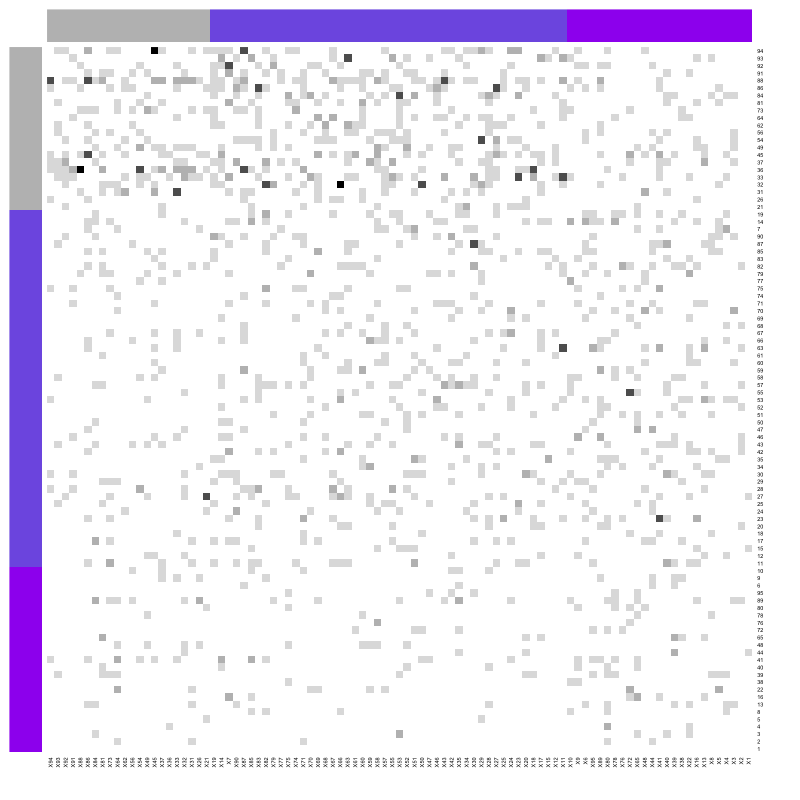
\includegraphics[width=.33\textwidth,natwidth=800,natheight=800]{/Users/lapo_santi/Desktop/Nial/POMM_pairwise/POMMs/Tennis application/results/processed_results/adjacency_Tennis_application_Est_model_POMM_K3_N95.png}%
        \label{fig:POMM_adjacency_K3}%
    }\hfill
    \subfigure[K=3, POMM Model]{%
        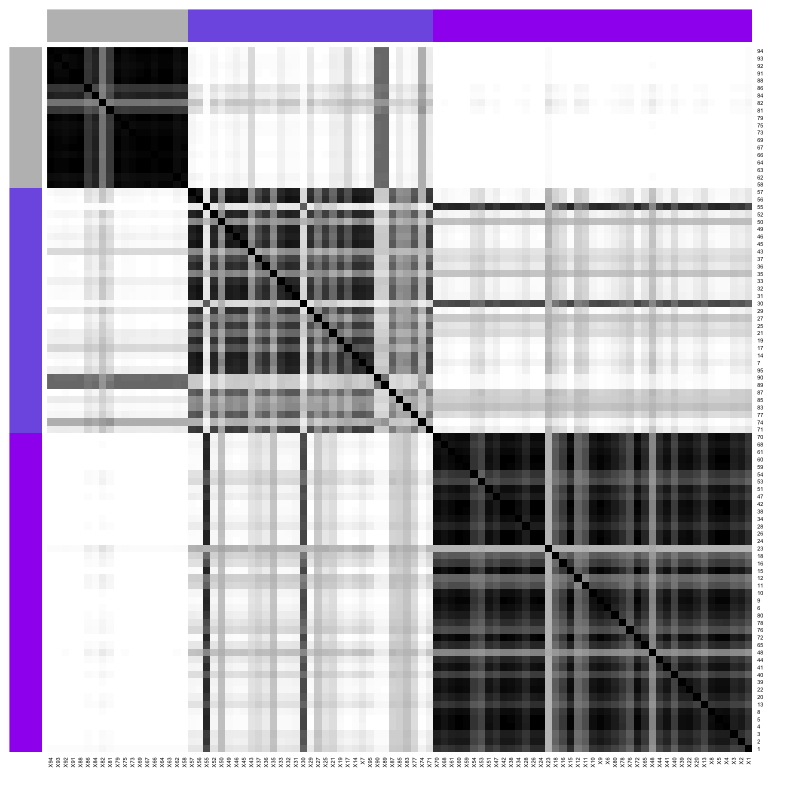
\includegraphics[width=.33\textwidth,natwidth=800,natheight=800]{/Users/lapo_santi/Desktop/Nial/POMM_pairwise/POMMs/Tennis application/results/processed_results/similarity_Tennis_application_Est_model_POMMK3_N95.png}%
        \label{fig:POMM_adjacency_K5}%
    }\hfill
    \subfigure[K=3, Simple Model]{%
        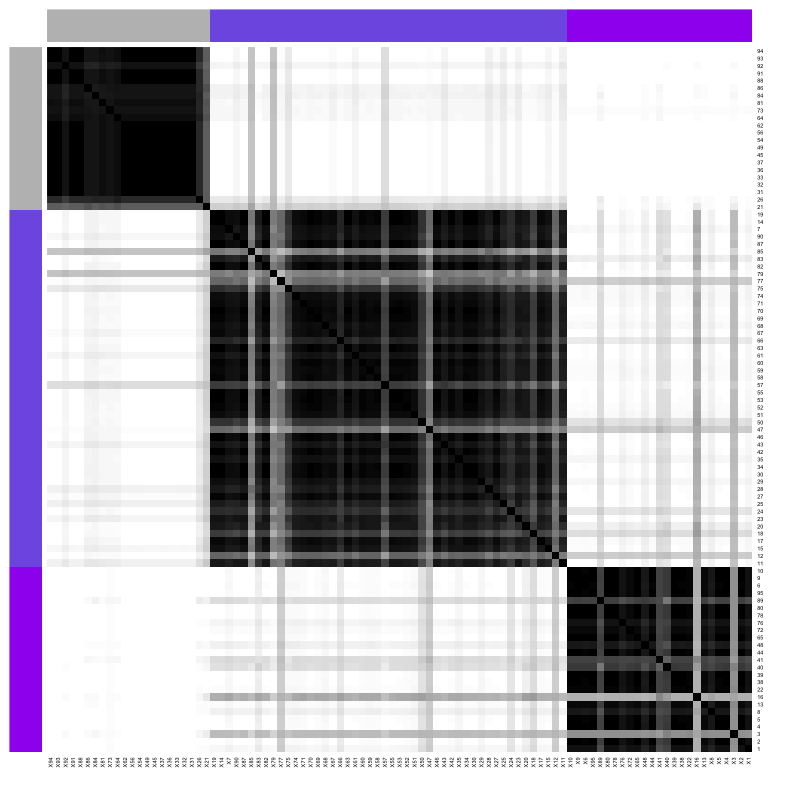
\includegraphics[width=.33\textwidth,natwidth=800,natheight=800]{/Users/lapo_santi/Desktop/Nial/POMM_pairwise/POMMs/Tennis application/results/processed_results/similarity_Tennis_application_Est_model_SimpleK3_N95.png}%
        \label{fig:POMM_adjacency_K9}%
    }
    \caption{Adjacency Matrices simulated via the POMM Model}
    \label{fig:all_images}
\end{figure}



















\clearpage

\section{Appendix I: Investigating Empirically the prior behaviour}


In this section, we explore the behaviour of the POMM prior, as $\alpha$, the parameter controlling the rate of increase of the power-law process and $S$, the variation (and therefore, the overlap) of the level sets sets, change. 

We start with a simulation study, whose results are reported in figure \eqref{fig}.

\begin{figure}[h]
    \centering
       \subfigure[$\alpha=0.1, S = 0.2$]{%
        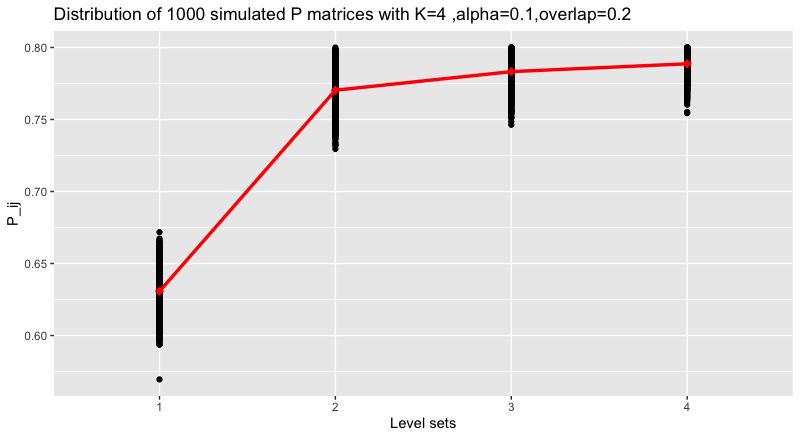
\includegraphics[width=.3333\textwidth,natwidth=800,natheight=438]{/Users/lapo_santi/Desktop/Nial/POMM_pairwise/POMMs/POMM_flex/exploratory_graphs_with_inference/alpha_and_overlap_investigation_alpha0.1overlap0.2K5.png}%
        \label{l}%
    }\hfill
    \subfigure[$\alpha=0.1, S = 0.4$]{%
        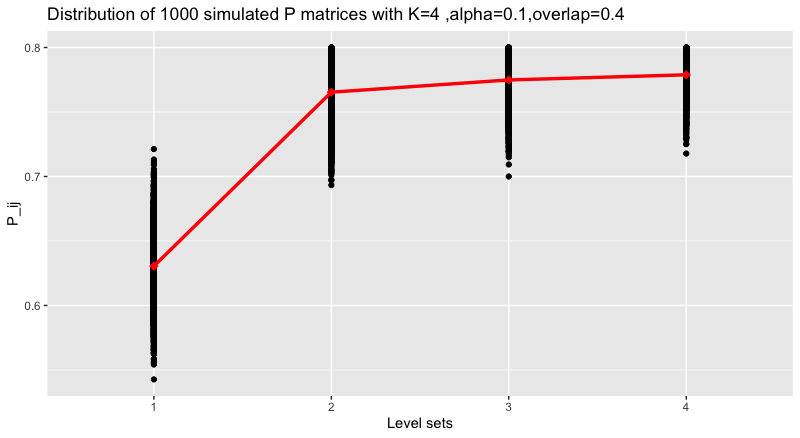
\includegraphics[width=.3333\textwidth,natwidth=800,natheight=438]{/Users/lapo_santi/Desktop/Nial/POMM_pairwise/POMMs/POMM_flex/exploratory_graphs_with_inference/alpha_and_overlap_investigation_alpha0.1overlap0.4K5.png}%
        \label{fig:M7000}%
    }\hfill
    \subfigure[$\alpha=0.1, S = 0.7$]{%
        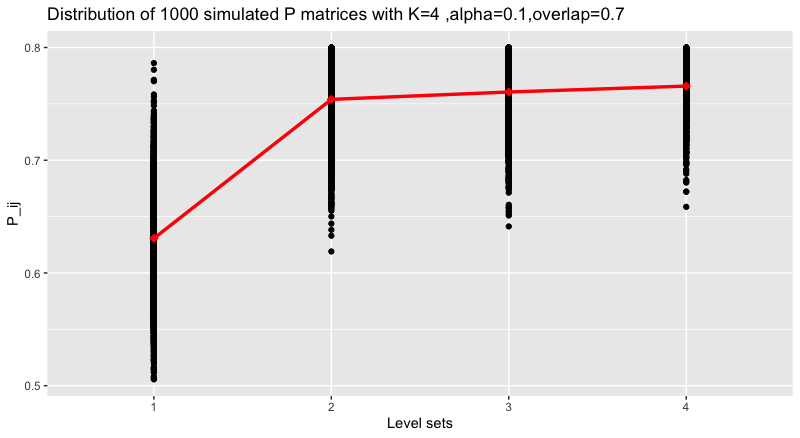
\includegraphics[width=.3333\textwidth,natwidth=800,natheight=438]{/Users/lapo_santi/Desktop/Nial/POMM_pairwise/POMMs/POMM_flex/exploratory_graphs_with_inference/alpha_and_overlap_investigation_alpha0.1overlap0.7K5.png}%
        \label{fig:M10000}%
    }\\[2ex]\subfigure[$\alpha=0.5, S = 0.2$]{%
        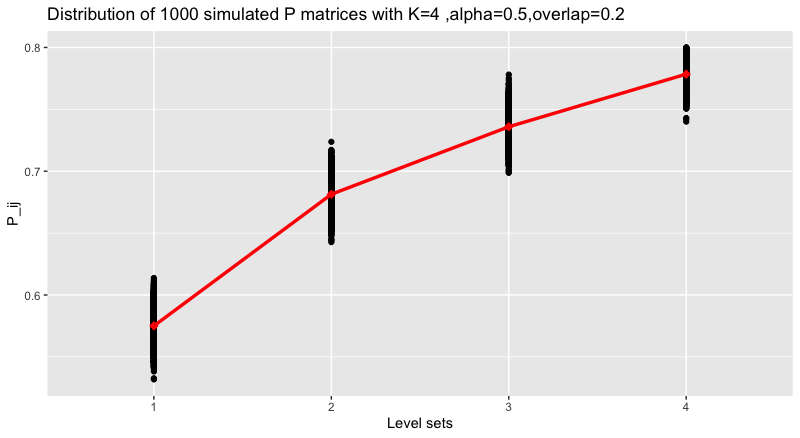
\includegraphics[width=.3333\textwidth,natwidth=800,natheight=438]{/Users/lapo_santi/Desktop/Nial/POMM_pairwise/POMMs/POMM_flex/exploratory_graphs_with_inference/alpha_and_overlap_investigation_alpha0.5overlap0.2K5.png}%
        \label{fig:M4000}%
    }\hfill
    \subfigure[$\alpha=0.5, S = 0.4$]{%
        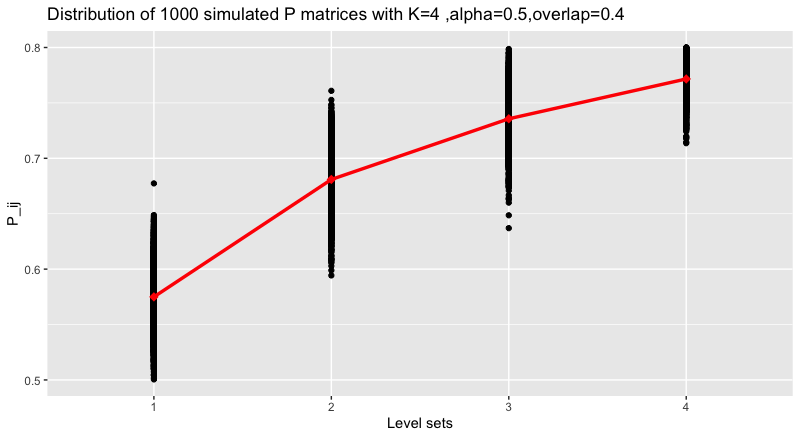
\includegraphics[width=.3333\textwidth,natwidth=800,natheight=438]{/Users/lapo_santi/Desktop/Nial/POMM_pairwise/POMMs/POMM_flex/exploratory_graphs_with_inference/alpha_and_overlap_investigation_alpha0.5overlap0.4K5.png}%
        \label{fig:M7000}%
    }\hfill
    \subfigure[$\alpha=0.5, S = 0.7$]{%
        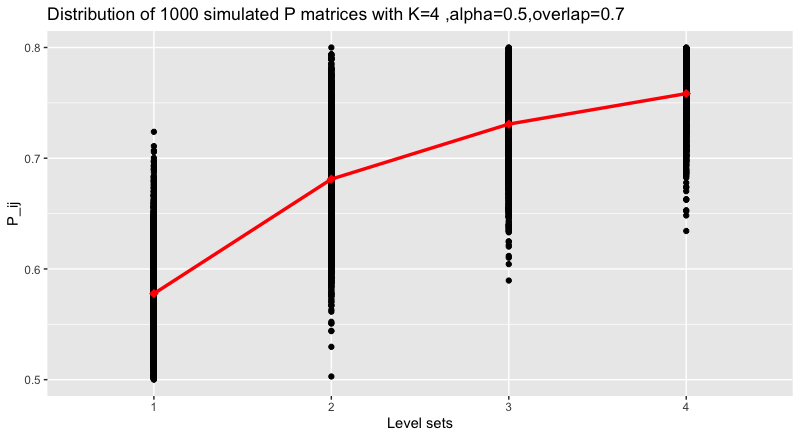
\includegraphics[width=.3333\textwidth,natwidth=800,natheight=438]{/Users/lapo_santi/Desktop/Nial/POMM_pairwise/POMMs/POMM_flex/exploratory_graphs_with_inference/alpha_and_overlap_investigation_alpha0.5overlap0.7K5.png}%
        \label{fig:M10000}%
    }\\[2ex]\subfigure[$\alpha=1, S = 0.2$]{%
        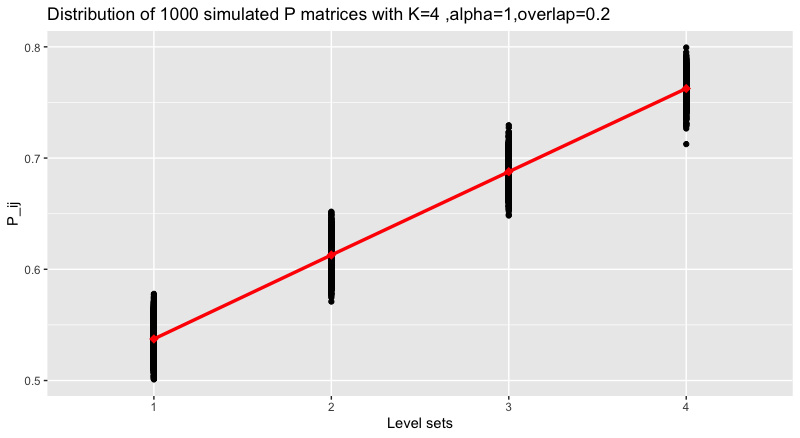
\includegraphics[width=.3333\textwidth,natwidth=800,natheight=438]{/Users/lapo_santi/Desktop/Nial/POMM_pairwise/POMMs/POMM_flex/exploratory_graphs_with_inference/alpha_and_overlap_investigation_alpha1overlap0.2K5.png}%
        \label{fig:M4000}%
    }\hfill
    \subfigure[$\alpha=1, S = 0.4$]{%
        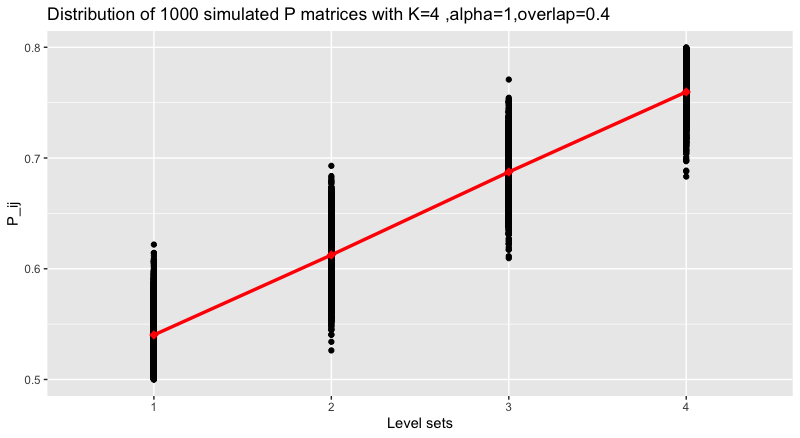
\includegraphics[width=.3333\textwidth,natwidth=800,natheight=438]{/Users/lapo_santi/Desktop/Nial/POMM_pairwise/POMMs/POMM_flex/exploratory_graphs_with_inference/alpha_and_overlap_investigation_alpha1overlap0.4K5.png}%
        \label{fig:M7000}%
    }\hfill
    \subfigure[$\alpha=1, S = 0.7$]{%
        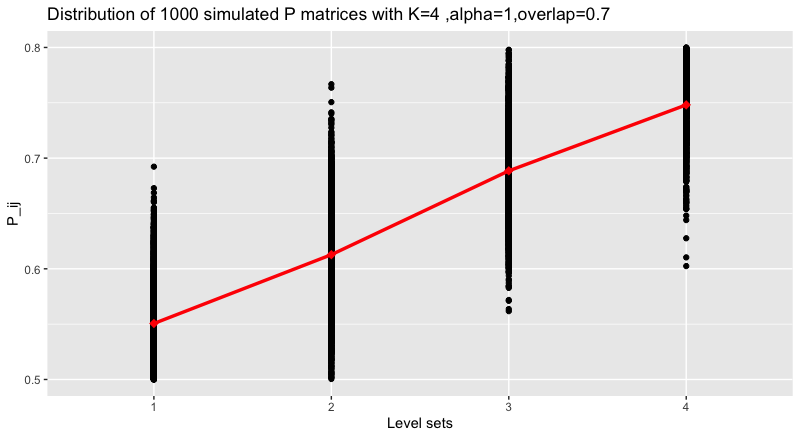
\includegraphics[width=.3333\textwidth,natwidth=800,natheight=438]{/Users/lapo_santi/Desktop/Nial/POMM_pairwise/POMMs/POMM_flex/exploratory_graphs_with_inference/alpha_and_overlap_investigation_alpha1overlap0.7K5.png}%
        \label{fig:M10000}%
    }\\[2ex]\subfigure[$\alpha=1.5, S = 0.2$]{%
        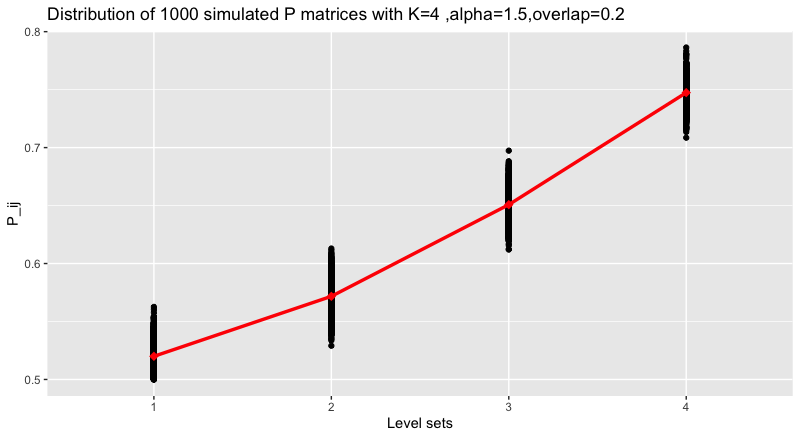
\includegraphics[width=.3333\textwidth,natwidth=800,natheight=438]{/Users/lapo_santi/Desktop/Nial/POMM_pairwise/POMMs/POMM_flex/exploratory_graphs_with_inference/alpha_and_overlap_investigation_alpha1.5overlap0.2K5.png}%
        \label{fig:M4000}%
    }\hfill
    \subfigure[$\alpha=1.5, S = 0.4$]{%
        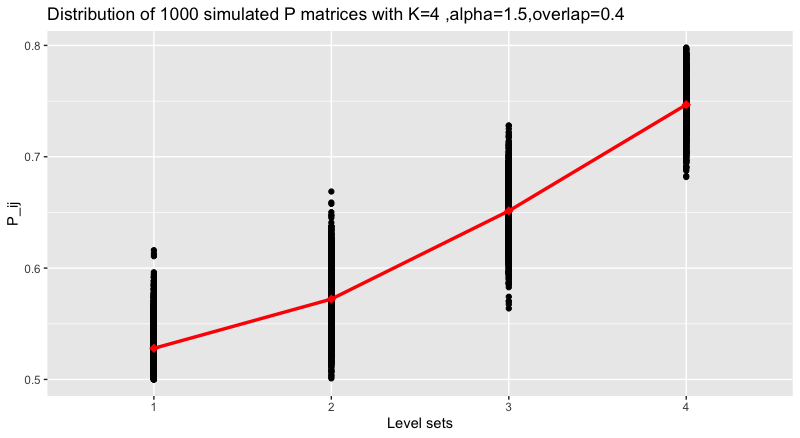
\includegraphics[width=.3333\textwidth,natwidth=800,natheight=438]{/Users/lapo_santi/Desktop/Nial/POMM_pairwise/POMMs/POMM_flex/exploratory_graphs_with_inference/alpha_and_overlap_investigation_alpha1.5overlap0.4K5.png}%
        \label{fig:M7000}%
    }\hfill
    \subfigure[$\alpha=1.5, S = 0.7$]{%
        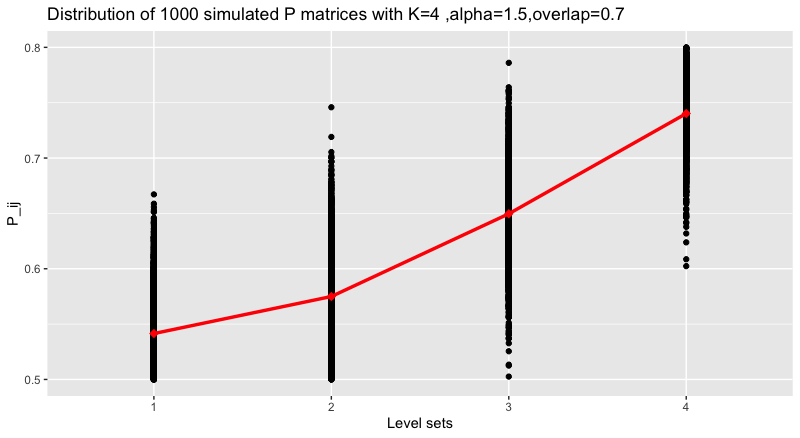
\includegraphics[width=.3333\textwidth,natwidth=800,natheight=438]{/Users/lapo_santi/Desktop/Nial/POMM_pairwise/POMMs/POMM_flex/exploratory_graphs_with_inference/alpha_and_overlap_investigation_alpha1.5overlap0.7K5.png}%
        \label{fig:M10000}%
    }\\[2ex]\subfigure[$\alpha=3, S = 0.2$]{%
        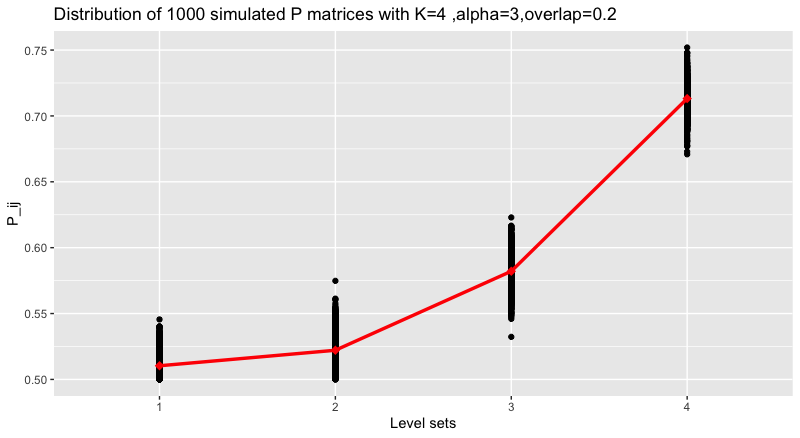
\includegraphics[width=.3333\textwidth,natwidth=800,natheight=438]{/Users/lapo_santi/Desktop/Nial/POMM_pairwise/POMMs/POMM_flex/exploratory_graphs_with_inference/alpha_and_overlap_investigation_alpha3overlap0.2K5.png}%
        \label{fig:M4000}%
    }\hfill
    \subfigure[$\alpha=3, S = 0.4$]{%
        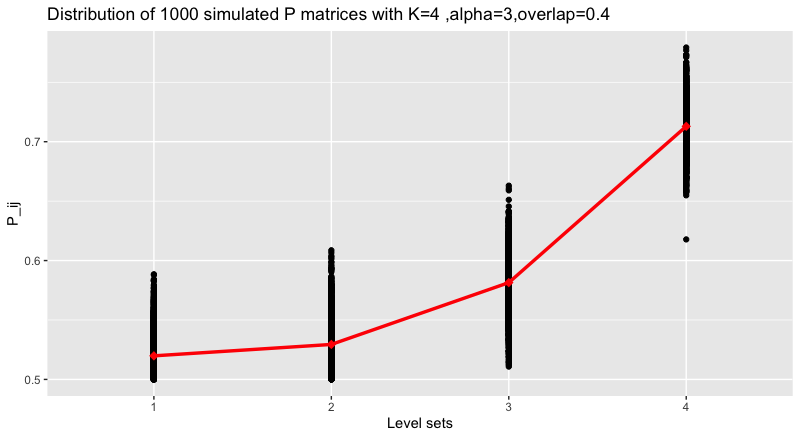
\includegraphics[width=.3333\textwidth,natwidth=800,natheight=438]{/Users/lapo_santi/Desktop/Nial/POMM_pairwise/POMMs/POMM_flex/exploratory_graphs_with_inference/alpha_and_overlap_investigation_alpha3overlap0.4K5.png}%
        \label{fig:M7000}%
    }\hfill
    \subfigure[$\alpha=3, S = 0.7$]{%
        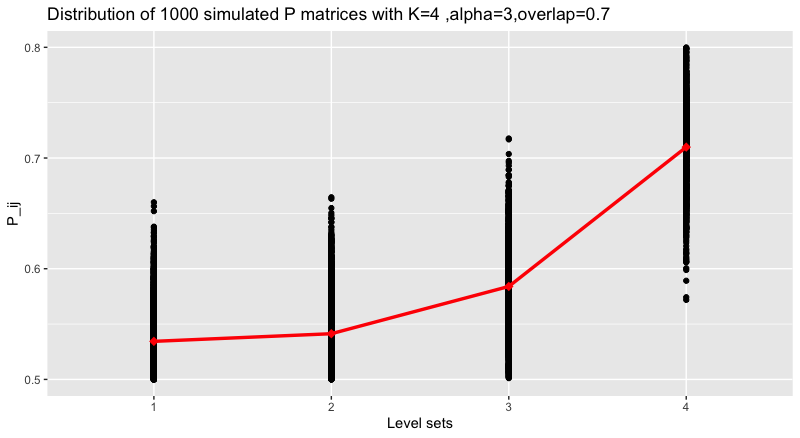
\includegraphics[width=.3333\textwidth,natwidth=800,natheight=438]{/Users/lapo_santi/Desktop/Nial/POMM_pairwise/POMMs/POMM_flex/exploratory_graphs_with_inference/alpha_and_overlap_investigation_alpha3overlap0.7K5.png}%
        \label{fig:M10000}%
    }
    \caption{Distribution of $n=1000$ simulated $P$ matrices with $\alpha \in \{0.1,0.5,1,1.5,3\}$ and $S \in \{0.2,0.4,0.7\}$. The points are grouped into the $K=5$ level sets- the main diagonal is set =0.5. The black vertical dots are the points, while the red lines show the evolution of the mean of the level sets.}
    \label{fig:exploratoryanalysisalpha_andS}
\end{figure}


\clearpage


\section{Appendix II: Empirical Assessment of the inference problem}

This section has two main objectives:

\begin{enumerate}
\item The first objective is to assess the identifiability of the POMM model. Given that the richness of the model, it is not obvious that the parameters are identifiable in all the regions of the parameter space. Therefore, by means of several simulation studies, we aim at identifying any possible identifiability constraints.
\item The second objective is code testing, by checking the whole estimation procedure on simulated data.
\end{enumerate}

\subsection{Focus on $\alpha$}
\begin{longtable}{l|rrr}
\caption{
{\large Mean absolute error for different alpha values} \\ 
{\small Sample size = 1000. MAEs = $|\hat{\alpha}_{\text{MLE}} - \alpha|$}
} \\ 
\toprule
\multicolumn{1}{l}{} & S = 0.2 & S = 0.4 & S = 0.7 \\ 
\midrule
$\alpha=$ 0.1 & $3.199 \times 10^{-4}$ & $1.270 \times 10^{-4}$ & $0.003$ \\ 
$\alpha=$ 0.5 & $1.377 \times 10^{-4}$ & $2.955 \times 10^{-4}$ & $0.001$ \\ 
$\alpha=$ 1.0 & $7.695 \times 10^{-4}$ & $0.007$ & $0.001$ \\ 
$\alpha=$ 1.5 & $0.001$ & $0.006$ & $0.004$ \\ 
$\alpha=$ 3.0 & $0.003$ & $0.036$ & $0.004$ \\ 
\bottomrule
\end{longtable}



\begin{figure}[h]
    \centering
       \subfigure[$\alpha=0.1, S = 0.2$]{%
        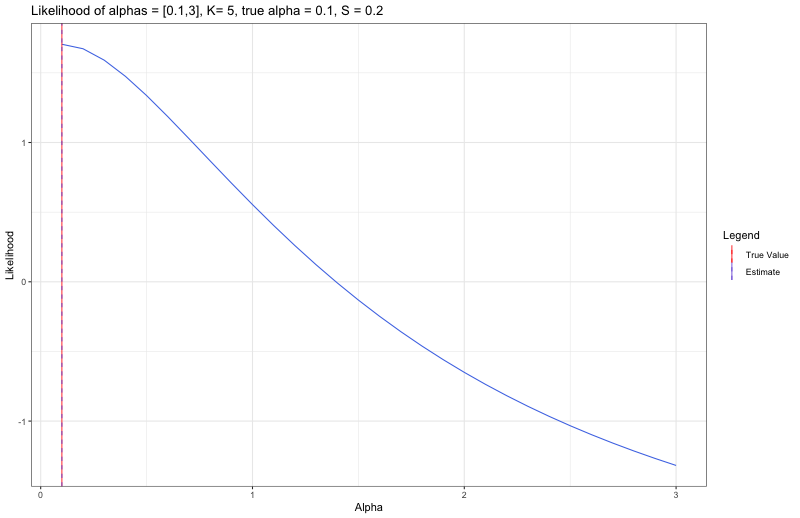
\includegraphics[width=.3333\textwidth,natwidth=800,natheight=438]{/Users/lapo_santi/Desktop/Nial/POMM_pairwise/POMMs/POMM_flex/exploratory_graphs_with_inference/LikelihoodK5_alpha0.1_overlap0.2_diag_.png}%
        \label{l}%
    }\hfill
    \subfigure[$\alpha=0.1, S = 0.4$]{%
        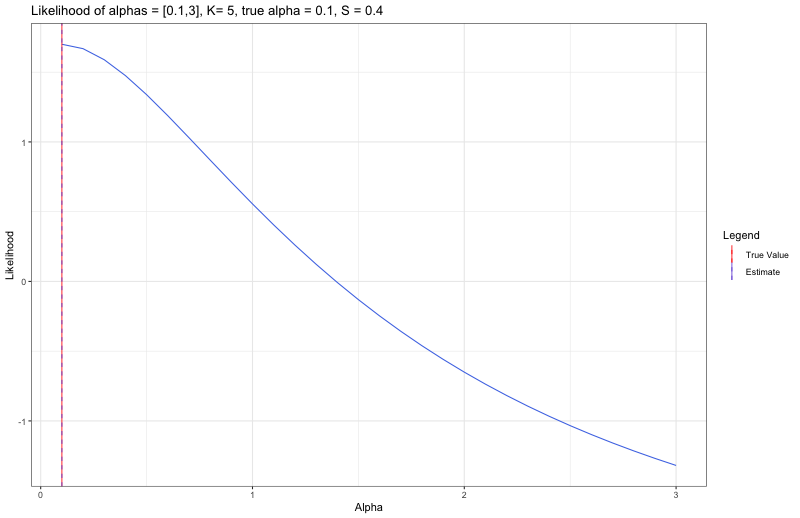
\includegraphics[width=.3333\textwidth,natwidth=800,natheight=438]{/Users/lapo_santi/Desktop/Nial/POMM_pairwise/POMMs/POMM_flex/exploratory_graphs_with_inference/LikelihoodK5_alpha0.1_overlap0.4_diag_.png}%
        \label{fig:M7000}%
    }\hfill
    \subfigure[$\alpha=0.1, S = 0.7$]{%
        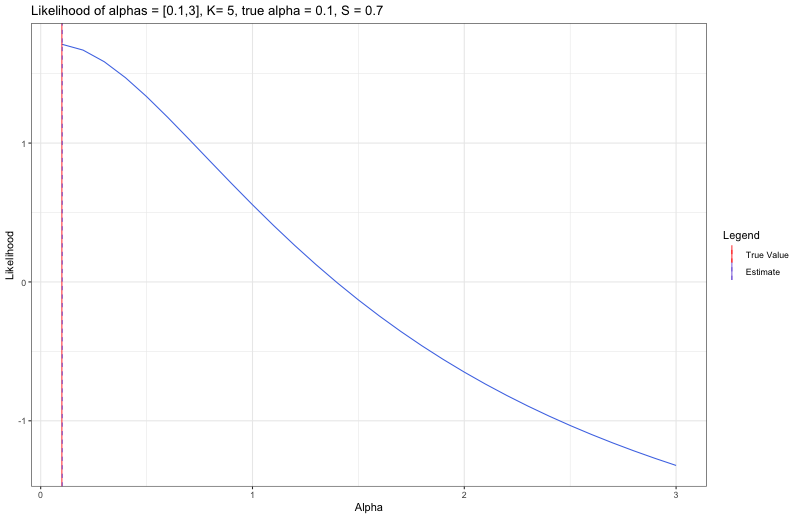
\includegraphics[width=.3333\textwidth,natwidth=800,natheight=438]{/Users/lapo_santi/Desktop/Nial/POMM_pairwise/POMMs/POMM_flex/exploratory_graphs_with_inference/LikelihoodK5_alpha0.1_overlap0.7_diag_.png}%
        \label{fig:M10000}%
    }\\[2ex]\subfigure[$\alpha=0.5, S = 0.2$]{%
        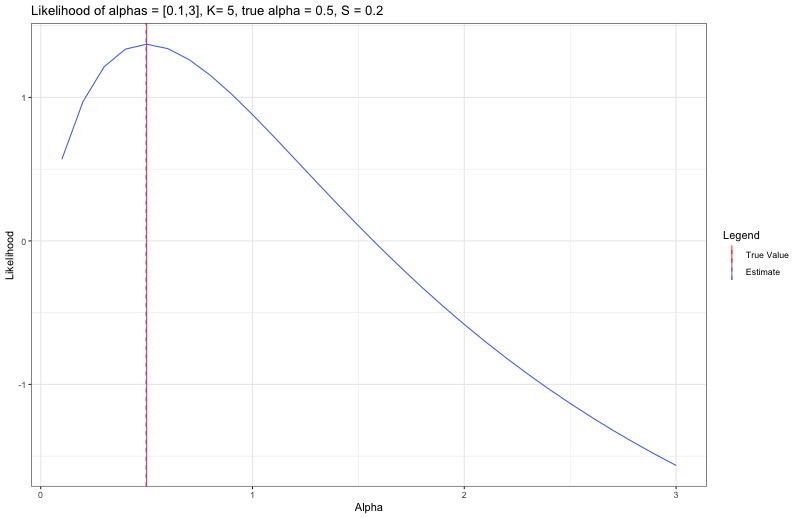
\includegraphics[width=.3333\textwidth,natwidth=800,natheight=438]{/Users/lapo_santi/Desktop/Nial/POMM_pairwise/POMMs/POMM_flex/exploratory_graphs_with_inference/LikelihoodK5_alpha0.5_overlap0.2_diag_.png}%
        \label{fig:M4000}%
    }\hfill
    \subfigure[$\alpha=0.5, S = 0.4$]{%
        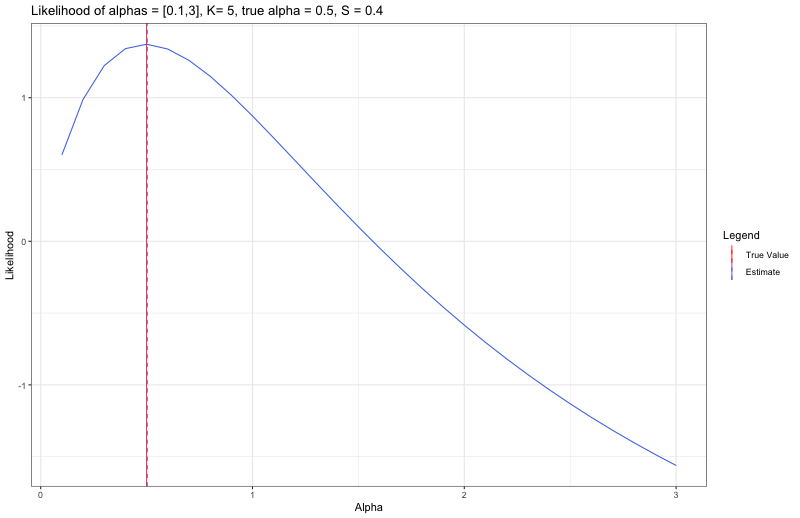
\includegraphics[width=.3333\textwidth,natwidth=800,natheight=438]{/Users/lapo_santi/Desktop/Nial/POMM_pairwise/POMMs/POMM_flex/exploratory_graphs_with_inference/LikelihoodK5_alpha0.5_overlap0.4_diag_.png}%
        \label{fig:M7000}%
    }\hfill
    \subfigure[$\alpha=0.5, S = 0.7$]{%
        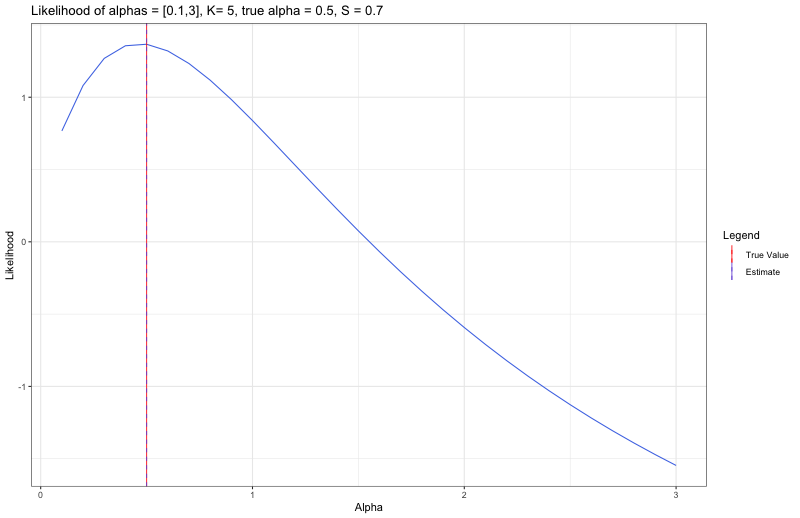
\includegraphics[width=.3333\textwidth,natwidth=800,natheight=438]{/Users/lapo_santi/Desktop/Nial/POMM_pairwise/POMMs/POMM_flex/exploratory_graphs_with_inference/LikelihoodK5_alpha0.5_overlap0.7_diag_.png}%
        \label{fig:M10000}%
    }\\[2ex]\subfigure[$\alpha=1, S = 0.2$]{%
        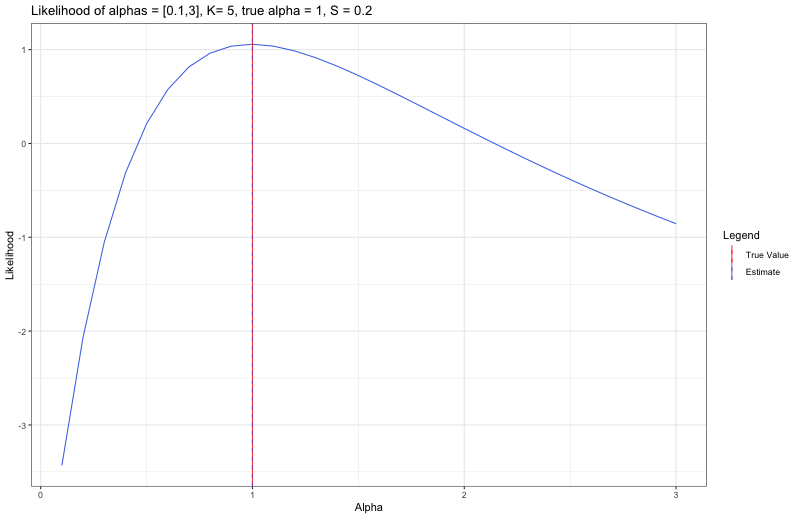
\includegraphics[width=.3333\textwidth,natwidth=800,natheight=438]{/Users/lapo_santi/Desktop/Nial/POMM_pairwise/POMMs/POMM_flex/exploratory_graphs_with_inference/LikelihoodK5_alpha1_overlap0.2_diag_.png}%
        \label{fig:M4000}%
    }\hfill
    \subfigure[$\alpha=1, S = 0.4$]{%
        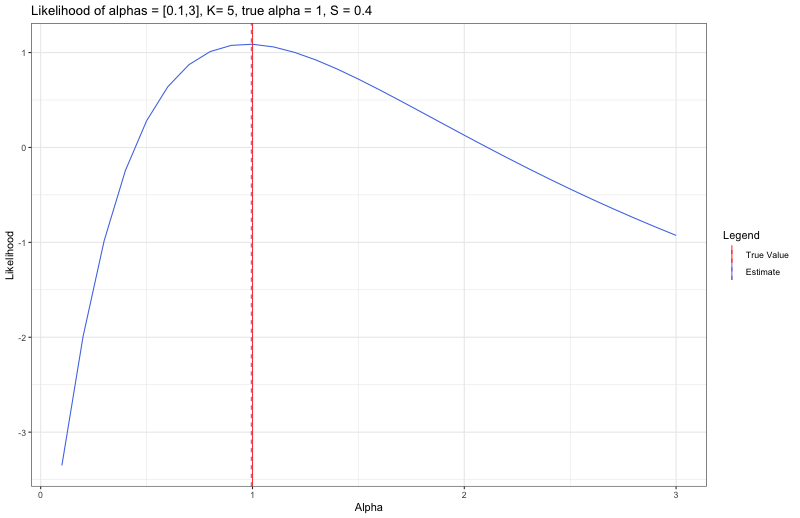
\includegraphics[width=.3333\textwidth,natwidth=800,natheight=438]{/Users/lapo_santi/Desktop/Nial/POMM_pairwise/POMMs/POMM_flex/exploratory_graphs_with_inference/LikelihoodK5_alpha1_overlap0.4_diag_.png}%
        \label{fig:M7000}%
    }\hfill
    \subfigure[$\alpha=1, S = 0.7$]{%
        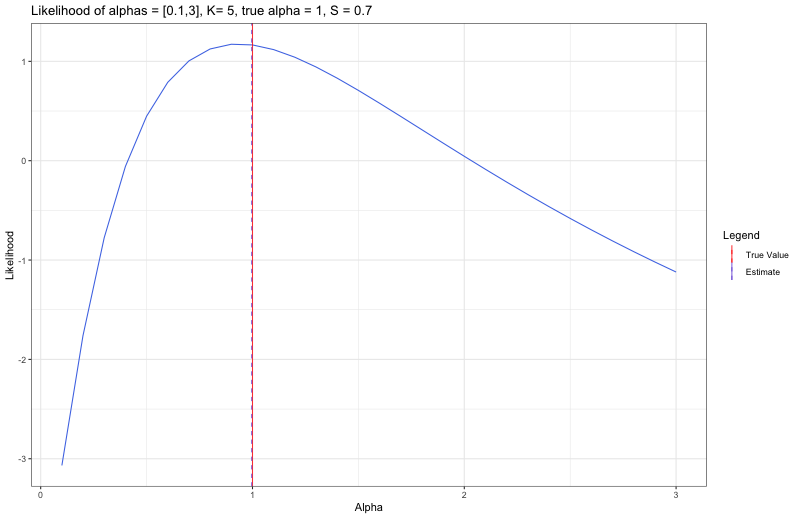
\includegraphics[width=.3333\textwidth,natwidth=800,natheight=438]{/Users/lapo_santi/Desktop/Nial/POMM_pairwise/POMMs/POMM_flex/exploratory_graphs_with_inference/LikelihoodK5_alpha1_overlap0.7_diag_.png}%
        \label{fig:M10000}%
    }\\[2ex]\subfigure[$\alpha=1.5, S = 0.2$]{%
        \includegraphics[width=.3333\textwidth,natwidth=800,natheight=438]{/Users/lapo_santi/Desktop/Nial/POMM_pairwise/POMMs/POMM_flex/exploratory_graphs_with_inference/LikelihoodK5_alpha1.5_overlap0.2_diag_.png}%
        \label{fig:M4000}%
    }\hfill
    \subfigure[$\alpha=1.5, S = 0.4$]{%
        \includegraphics[width=.3333\textwidth,natwidth=800,natheight=438]{/Users/lapo_santi/Desktop/Nial/POMM_pairwise/POMMs/POMM_flex/exploratory_graphs_with_inference/LikelihoodK5_alpha1.5_overlap0.4_diag_.png}%
        \label{fig:M7000}%
    }\hfill
    \subfigure[$\alpha=1.5, S = 0.7$]{%
        \includegraphics[width=.3333\textwidth,natwidth=800,natheight=438]{/Users/lapo_santi/Desktop/Nial/POMM_pairwise/POMMs/POMM_flex/exploratory_graphs_with_inference/LikelihoodK5_alpha1.5_overlap0.7_diag_.png}%
        \label{fig:M10000}%
    }\\[2ex]\subfigure[$\alpha=3, S = 0.2$]{%
        \includegraphics[width=.3333\textwidth,natwidth=800,natheight=438]{/Users/lapo_santi/Desktop/Nial/POMM_pairwise/POMMs/POMM_flex/exploratory_graphs_with_inference/LikelihoodK5_alpha3_overlap0.2_diag_.png}%
        \label{fig:M4000}%
    }\hfill
    \subfigure[$\alpha=3, S = 0.4$]{%
        \includegraphics[width=.3333\textwidth,natwidth=800,natheight=438]{/Users/lapo_santi/Desktop/Nial/POMM_pairwise/POMMs/POMM_flex/exploratory_graphs_with_inference/LikelihoodK5_alpha3_overlap0.4_diag_.png}%
        \label{fig:M7000}%
    }\hfill
    \subfigure[$\alpha=3, S = 0.7$]{%
        \includegraphics[width=.3333\textwidth,natwidth=800,natheight=438]{/Users/lapo_santi/Desktop/Nial/POMM_pairwise/POMMs/POMM_flex/exploratory_graphs_with_inference/LikelihoodK5_alpha3_overlap0.7_diag_.png}%
        \label{fig:M10000}%
    }
    \caption{Distribution of $n=1000$ simulated $P$ matrices with $\alpha \in \{0.1,0.5,1,1.5,3\}$ and $S \in \{0.2,0.4,0.7\}$. The points are grouped into the $K=5$ level sets- the main diagonal is set =0.5. The black vertical dots are the points, while the red lines show the evolution of the mean of the level sets.}
    \label{fig:exploratoryanalysisalpha_andS}
\end{figure}


\subsubsection{Updating $\alpha$ algorithm}

3


\subsubsection{Montecarlo algorithm}



\subsection{Focus on $S$}

\begin{longtable}{l|rrrrr}
\caption*{
{\large Mean absolute error for different $S$ values} \\ 
{\small Each row is a different $S$ value. Sample size = 1000}
} \\ 
\toprule
\multicolumn{1}{l}{} & $\alpha = 0.1$ & $\alpha = 0.5$ & $\alpha = 1$ & $\alpha = 1.5$ & $\alpha = 3$ \\ 
\midrule
S = 0.2 & $0.002$ & $0.002$ & $9.780 \times 10^{-4}$ & $3.709 \times 10^{-4}$ & $9.931 \times 10^{-4}$ \\ 
S = 0.4 & $0.005$ & $0.003$ & $0.006$ & $0.002$ & $0.003$ \\ 
S = 0.7 & $0.006$ & $0.002$ & $0.005$ & $0.006$ & $0.007$ \\ 
\bottomrule
\end{longtable}


\begin{figure}[h]
    \centering
       \subfigure[$\alpha=0.1, S = 0.2$]{%
        \includegraphics[width=.3333\textwidth,natwidth=800,natheight=438]{/Users/lapo_santi/Desktop/Nial/POMM_pairwise/POMMs/POMM_flex/exploratory_graphs_with_inference/Overlap_LikelihoodK5_alpha0.1_overlap0.2_diag_.png}%
        \label{l}%
    }\hfill
    \subfigure[$\alpha=0.1, S = 0.4$]{%
        \includegraphics[width=.3333\textwidth,natwidth=800,natheight=438]{/Users/lapo_santi/Desktop/Nial/POMM_pairwise/POMMs/POMM_flex/exploratory_graphs_with_inference/Overlap_LikelihoodK5_alpha0.1_overlap0.4_diag_.png}%
        \label{fig:M7000}%
    }\hfill
    \subfigure[$\alpha=0.1, S = 0.7$]{%
        \includegraphics[width=.3333\textwidth,natwidth=800,natheight=438]{/Users/lapo_santi/Desktop/Nial/POMM_pairwise/POMMs/POMM_flex/exploratory_graphs_with_inference/Overlap_LikelihoodK5_alpha0.1_overlap0.7_diag_.png}%
        \label{fig:M10000}%
    }\\[2ex]\subfigure[$\alpha=0.5, S = 0.2$]{%
        \includegraphics[width=.3333\textwidth,natwidth=800,natheight=438]{/Users/lapo_santi/Desktop/Nial/POMM_pairwise/POMMs/POMM_flex/exploratory_graphs_with_inference/Overlap_LikelihoodK5_alpha0.5_overlap0.2_diag_.png}%
        \label{fig:M4000}%
    }\hfill
    \subfigure[$\alpha=0.5, S = 0.4$]{%
        \includegraphics[width=.3333\textwidth,natwidth=800,natheight=438]{/Users/lapo_santi/Desktop/Nial/POMM_pairwise/POMMs/POMM_flex/exploratory_graphs_with_inference/Overlap_LikelihoodK5_alpha0.5_overlap0.4_diag_.png}%
        \label{fig:M7000}%
    }\hfill
    \subfigure[$\alpha=0.5, S = 0.7$]{%
        \includegraphics[width=.3333\textwidth,natwidth=800,natheight=438]{/Users/lapo_santi/Desktop/Nial/POMM_pairwise/POMMs/POMM_flex/exploratory_graphs_with_inference/Overlap_LikelihoodK5_alpha0.5_overlap0.7_diag_.png}%
        \label{fig:M10000}%
    }\\[2ex]\subfigure[$\alpha=1, S = 0.2$]{%
        \includegraphics[width=.3333\textwidth,natwidth=800,natheight=438]{/Users/lapo_santi/Desktop/Nial/POMM_pairwise/POMMs/POMM_flex/exploratory_graphs_with_inference/Overlap_LikelihoodK5_alpha1_overlap0.2_diag_.png}%
        \label{fig:M4000}%
    }\hfill
    \subfigure[$\alpha=1, S = 0.4$]{%
        \includegraphics[width=.3333\textwidth,natwidth=800,natheight=438]{/Users/lapo_santi/Desktop/Nial/POMM_pairwise/POMMs/POMM_flex/exploratory_graphs_with_inference/Overlap_LikelihoodK5_alpha1_overlap0.4_diag_.png}%
        \label{fig:M7000}%
    }\hfill
    \subfigure[$\alpha=1, S = 0.7$]{%
        \includegraphics[width=.3333\textwidth,natwidth=800,natheight=438]{/Users/lapo_santi/Desktop/Nial/POMM_pairwise/POMMs/POMM_flex/exploratory_graphs_with_inference/Overlap_LikelihoodK5_alpha1_overlap0.7_diag_.png}%
        \label{fig:M10000}%
    }\\[2ex]\subfigure[$\alpha=1.5, S = 0.2$]{%
        \includegraphics[width=.3333\textwidth,natwidth=800,natheight=438]{/Users/lapo_santi/Desktop/Nial/POMM_pairwise/POMMs/POMM_flex/exploratory_graphs_with_inference/Overlap_LikelihoodK5_alpha1.5_overlap0.2_diag_.png}%
        \label{fig:M4000}%
    }\hfill
    \subfigure[$\alpha=1.5, S = 0.4$]{%
        \includegraphics[width=.3333\textwidth,natwidth=800,natheight=438]{/Users/lapo_santi/Desktop/Nial/POMM_pairwise/POMMs/POMM_flex/exploratory_graphs_with_inference/Overlap_LikelihoodK5_alpha1.5_overlap0.4_diag_.png}%
        \label{fig:M7000}%
    }\hfill
    \subfigure[$\alpha=1.5, S = 0.7$]{%
        \includegraphics[width=.3333\textwidth,natwidth=800,natheight=438]{/Users/lapo_santi/Desktop/Nial/POMM_pairwise/POMMs/POMM_flex/exploratory_graphs_with_inference/Overlap_LikelihoodK5_alpha1.5_overlap0.7_diag_.png}%
        \label{fig:M10000}%
    }\\[2ex]\subfigure[$\alpha=3, S = 0.2$]{%
        \includegraphics[width=.3333\textwidth,natwidth=800,natheight=438]{/Users/lapo_santi/Desktop/Nial/POMM_pairwise/POMMs/POMM_flex/exploratory_graphs_with_inference/Overlap_LikelihoodK5_alpha3_overlap0.2_diag_.png}%
        \label{fig:M4000}%
    }\hfill
    \subfigure[$\alpha=3, S = 0.4$]{%
        \includegraphics[width=.3333\textwidth,natwidth=800,natheight=438]{/Users/lapo_santi/Desktop/Nial/POMM_pairwise/POMMs/POMM_flex/exploratory_graphs_with_inference/Overlap_LikelihoodK5_alpha3_overlap0.4_diag_.png}%
        \label{fig:M7000}%
    }\hfill
    \subfigure[$\alpha=3, S = 0.7$]{%
        \includegraphics[width=.3333\textwidth,natwidth=800,natheight=438]{/Users/lapo_santi/Desktop/Nial/POMM_pairwise/POMMs/POMM_flex/exploratory_graphs_with_inference/Overlap_LikelihoodK5_alpha3_overlap0.7_diag_.png}%
        \label{fig:M10000}%
    }
    \caption{Distribution of $n=1000$ simulated $P$ matrices with $\alpha \in \{0.1,0.5,1,1.5,3\}$ and $S \in \{0.2,0.4,0.7\}$. The points are grouped into the $K=5$ level sets- the main diagonal is set =0.5. The black vertical dots are the points, while the red lines show the evolution of the mean of the level sets.}
    \label{fig:exploratoryanalysisalpha_andS}
\end{figure}


\subsubsection{Montecarlo algorithm}


\begin{comment}

\begin{comment}

\section{ATP tennis dataset}


Our raw data are in a repository which can be found at \begin{center}\texttt{'https://pkgstore.datahub.io/sports-data/atp-world-tour-tennis-data'}\end{center}. If two players have played multiple times, they compare on different rows as we can see in Table(1). 

\begin{table}
\begin{center}\begin{tabular}{cccc} $\textbf{Winner}$ & $\textbf{Loser}$ \\Djockovic & Medvedev \\ \vdots & \vdots \\Djockovic & Medvedev  \\Djockovic & Medvedev \\ Medvedev & Djockovic \\\vdots & \vdots \\ Medvedev & Djockovic \\ Medvedev & Djockovic  \end{tabular} \caption{Raw data}
\end{center}
\label{Raw data}
\end{table}

To begin with, we select all rows with the first pair of players, regardless of the order in which they appear. Then, we construct these two new variables:
\begin{itemize}
\item $n_{games}$: the total number of games between player A and player B, which can be calculated as the sum of the number of victories of player A against player B and the number of victories of player B against player A. Basically, one counts the number of times these two names appear on the same row, irrespective of their order.
\item $n_{victories}$: the total number of victories of player A against player B, which can be calculated as the number of times player A appears before player B on the same row.
\end{itemize}

Then, I retain just the first pair observation, e.g. player A and player B, and disregard all the others. This process is repeated for all unique unordered pairs of players. In this way, I obtain a dataset storing, for each pair of players who have played at least once, all the relevant information in one single entry.

What about the observations in which player B won against player A? These will no longer be entries in the dataframe. However, this data will still be indirectly available by computing the total number of games between player A and player B (available in column $n_{games}$, at the corresponding row) minus the total number of victories of player A against player B (available in $n_{victories}$, at the corresponding row).

The final dataframe will look like as in Table (2).
\begin{table}
\begin{center}\begin{tabular}{cccc} $\textbf{Player1}$ & $\textbf{Player2}$ & $n_{games}$ & $n_{victories}$ \\Djockovic & Medvedev & 5 & 3 \\Djockovic & Nadal & 8 & 6 \\Nadal & Tsonga & 4 & 0\end{tabular} \caption{Final dataset}
\end{center}
\label{Final dataset}
\end{table}

\clearpage

\section{Descriptive statistics comparing simulated vs ATP data}


We start by choosing a particular configuration of parameters to simulate a given tournament to compare it with the ATP data.
\begin{itemize}
\item \texttt{N}=537 since in the ATP dataset we have exactly 537 players
\item \texttt{M}=3389 since in the ATP dataset this is the total number of matches
\item \texttt{max\_number\_games} = 4 since this is the max value we observe in the ATP data.
\end{itemize}
So, for these three initial parameters, we are replicating the features of the real tennis data. With respect to the more "statistical" ones there is no benchmark, so we choose to follow the intuition:
\begin{itemize}
\item \texttt{max\_clust}=3
\item \texttt{min\_clust}=3
\item \texttt{c} = 1.7
\item \texttt{beta\_max} = .8
\end{itemize}
After generating the data, we compare the simulated tournament and the true ATP data by computing some summary statistics and some meaningful plots shown in Figures (\ref{fig:scatterplot}), (\ref{fig:boxplotnij}), (\ref{fig:densityplotnij}), (\ref{fig:boxplotyij}), (\ref{fig:densityplotyij}). The scatterplot shows a similar pattern of strong correlation between $y_{ij}$ and $n_{ij}$. However, in ATP there is a higher points density close to the origin, while in the simulated tournament we have more density close to the mean. It means that real data are more dispersed than simulated ones. We can reach the same conclusion by looking at the number of games distribution and the number of victories. In particular, by looking at Figures (\ref{fig:boxplotyij}) and (\ref{fig:densityplotyij}) the discrepancy seems more enhanced for the number of victories $y_{ij}$. 

The interesting aspect of this methodology is that we could compute the discrepancy between the two distributions, for example using a Kullback-Leibler divergence, and find those parameters that minimize it.

\begin{figure}
\begin{minipage}{.8\textwidth}
      \centering
\includegraphics[width=.5\textwidth,natwidth=400,natheight=330]{/Users/lapo_santi/Desktop/Nial/project/descriptive statistic/comparison statistics/Scatterplot.png}
\caption{Scatterplot of $n_{ij}$, the number of games played between any two pair of players, and $y_{ij}$, the number of victories of player $i$ vs player $j$. We show the values both for Simulated (blue) and ATP data (red)}
\label{fig:scatterplot}
\end{minipage}\hfill
    \centering
    \begin{minipage}{0.25\textwidth}
        \centering
\includegraphics[width=\textwidth,natwidth=400,natheight=330]{/Users/lapo_santi/Desktop/Nial/project/descriptive statistic/comparison statistics/boxplotnij.png}
        \caption{Boxplot of $n_{ij}$ values both for Simulated (blue) and ATP data (red)}
        \label{fig:boxplotnij}
    \end{minipage}
    \begin{minipage}{0.25\textwidth}
        \centering
        \includegraphics[width=\textwidth,natwidth=400,natheight=330]{/Users/lapo_santi/Desktop/Nial/project/descriptive statistic/comparison statistics/densityplotnij.png}
        \caption{Density Plot for the $n_{ij}$ values both for Simulated (blue) and ATP data (red)}
        \label{fig:densityplotnij}
    \end{minipage}
    \vskip\floatsep
    \begin{minipage}{0.25\textwidth}
        \centering
 \includegraphics[width=\textwidth,natwidth=400,natheight=330]{/Users/lapo_santi/Desktop/Nial/project/descriptive statistic/comparison statistics/boxplotyij.png}
        \caption{Boxplot of $y_{ij}$ values both for Simulated (blue) and ATP data (red)}
        \label{fig:boxplotyij}
    \end{minipage}
    \begin{minipage}{0.25\textwidth}
        \centering
        \includegraphics[width=\textwidth,natwidth=400,natheight=330]{/Users/lapo_santi/Desktop/Nial/project/descriptive statistic/comparison statistics/densityplotyij.png}
        \caption{Density Plot for the $n_{ij}$ values both for Simulated (blue) and ATP data (red)}
        \label{fig:densityplotyij}
    \end{minipage}
\end{figure}



\end{comment}







\clearpage

\section{Appendix I: Estimation Details}


\subsection{Updating z}

To update $z$ we propose a new label for each node, we evaluate the accept/reject move by computing the ratio $r$ as follows:
\begin{align}
r &= \frac{\prod_{i<j}\binom{n_{ij}}{y_{ij}}p_{z^{\prime}_i z^{\prime}_j}^{y_{ij}} \cdot (1 - p_{z^{\prime}_i z^{\prime}_j})^{n_{ij} - y_{ij}} \cdot \frac{\Gamma(\gamma_0) \Gamma(n+1)}{\Gamma(n + \gamma_0)} \cdot \prod_{k=1}^K \frac{\Gamma(n^{\prime}_k + \gamma_k)}{\Gamma(\gamma_k)  \Gamma(n^{\prime}_k + 1)}}{\prod_{i<j}\binom{n_{ij}}{y_{ij}}p_{z_iz_j}^{y_{ij}} \cdot (1 - p_{z_iz_j})^{n_{ij} - y_{ij}}\cdot \frac{\Gamma(\gamma_0) \Gamma(n+1)}{\Gamma(n + \gamma_0)} \cdot \prod_{k=1}^K \frac{\Gamma(n_k + \gamma_k)}{\Gamma(\gamma_k)  \Gamma(n_k + 1)}} \\
 &= \frac{\prod_{i<j}p_{z^{\prime}_i z^{\prime}_j}^{y_{ij}} \cdot (1 - p_{z^{\prime}_i z^{\prime}_j})^{n_{ij} - y_{ij}} \cdot  \prod_{k=1}^K \frac{\Gamma(n^{\prime}_k + \gamma_k)}{\Gamma(\gamma_k)  \Gamma(n^{\prime}_k + 1)}}{\prod_{i<j}p_{z_iz_j}^{y_{ij}} \cdot (1 - p_{z_iz_j})^{n_{ij} - y_{ij}} \cdot \prod_{k=1}^K \frac{\Gamma(n_k + \gamma_k)}{\Gamma(\gamma_k)  \Gamma(n_k + 1)}} 
\end{align}


Passing to the log:

\begin{align}
log(r) &= \log{ \left( \prod_{i<j}p_{z^{\prime}_i z^{\prime}_j}^{y_{ij}} \cdot (1 - p_{z^{\prime}_i z^{\prime}_j})^{n_{ij} - y_{ij}} \cdot  \prod_{k=1}^K \frac{\Gamma(n^{\prime}_k + \gamma_k)}{\Gamma(\gamma_k)  \Gamma(n^{\prime}_k + 1)} \right) }  \nonumber \\
& \qquad - \log{ \left( \prod_{i<j}p_{z_iz_j}^{y_{ij}} \cdot (1 - p_{z_iz_j})^{n_{ij} - y_{ij}} \cdot \prod_{k=1}^K \frac{\Gamma(n_k + \gamma_k)}{\Gamma(\gamma_k)  \Gamma(n_k + 1)}\right)} \nonumber \\
&= \sum_{i<j} \left(   y_{ij} \cdot \log{ p_{z^{\prime}_i z^{\prime}_j} } + (n_{ij} - y_{ij}) \cdot \log{ (1 - p_{z^{\prime}_i z^{\prime}_j}) } \right)\nonumber \\ 
&\qquad +  \sum_{k=1}^K\left(\log\left(\Gamma(n^{\prime}_{k}+\gamma_{k})\right) - \log\left(\Gamma(\gamma_{k})\right) - \log\left(\Gamma\left(n^{\prime}_{k}+1\right)\right) \right)  \nonumber  \\
& \qquad \qquad - \sum_{i<j} \left(  y_{ij} \cdot \log{ p_{z_i z_j} } + (n_{ij} - y_{ij}) \cdot \log{ (1 - p_{z_i z_j}) } \right) \nonumber \\
&\qquad \qquad \qquad - \sum_{k=1}^K\left(\log\left(\Gamma(n_{k}+\gamma_{k})\right) - \log\left(\Gamma(\gamma_{k})\right) - \log\left(\Gamma\left(n_{k}+1\right)\right) \right) \nonumber \\
\end{align}


\begin{algorithm}
\begin{algorithmic}[1]
\For{$i \gets 1$ to $N$}
\State Sample $\texttt{new\_label}$ from $1,...,K$
\State Set $z^{\prime} \gets z$ with the $i$-th element replaced by $\texttt{new\_label}$
\State Compute new victory probabilities $p_{z^{\prime}_i z^{\prime}_j}$ using $z^{\prime}$
\State Compute probability ratio $log(r)$  using $p_{z^{\prime}_i z^{\prime}_j}$ and $p_{z_i z_j}$
\State Set $\alpha_{r} \gets \min(1, r)$
\State Sample $u$ from a uniform distribution on $(0,1)$
\If{$u < \alpha_{r}$}
\State Update $z$ to $z^{\prime}$
\State Update $p_{z_iz_j}$ to $p_{z^{\prime}_i z^{\prime}_j}$
\State Increment $acc.count_{z}$
\EndIf
\State Store $z_{current}$ in $z.container$
\EndFor
\end{algorithmic}
\label{alg:z_update}
\caption{Updating $z$ step}
\end{algorithm}


\subsection{Updating $\mathbf{P}$}


To update $P$ and $\alpha$ we propose a new label for each node, we evaluate the accept/reject move by computing the ratio $r$ as follows:

\begin{align}
r &= \frac{\prod_{i<j}\binom{n_{ij}}{y_{ij}}p_{z_i z_j}^{\prime y_{ij}} \cdot (1 - p^{\prime}_{z_i z_j})^{n_{ij} - y_{ij}} \cdot \prod_{k=1}^K  \left( \frac{1}{y^{\prime (k+1)} - y^{\prime(k)}}\right)^{|L^{\prime(k)}|}}{\prod_{i<j}\binom{n_{ij}}{y_{ij}}p_{z_i z_j}^{y_{ij}} \cdot (1 - p_{z_i z_j})^{n_{ij} - y_{ij}} \cdot \prod_{k=1}^K  \left( \frac{1}{y^{(k+1)} - y^{(k)}}\right)^{|L^{(k)}|}} \\
\end{align}


Passing to the log:

\begin{align}
log(r) &= \sum_{i<j} \left(  y_{ij} \cdot \log{ p^{\prime}_{z_i z_j} } + (n_{ij} - y_{ij}) \cdot \log{ (1 - p^{\prime}_{z_i z_j}) } \right)  - \sum_{k=1}^K |L^{\prime(k)}| \cdot \log{\left( y^{\prime(k+1)} - y^{\prime(k)} \right)}\\
 &\qquad - \sum_{i<j} \left(  y_{ij} \cdot \log{ p_{z_i z_j} } + (n_{ij} - y_{ij}) \cdot \log{ (1 - p_{z_i z_j}) } \right)  + \sum_{k=1}^K |L^{(k)}| \cdot \log{\left( y^{(k+1)} - y^{(k)} \right) }
\end{align}







\begin{algorithm}
\begin{algorithmic}[1]
\State $j \gets 1$
\While{$j \leq N_{iter}$}
\State Sample $\alpha^{\prime}$ from a truncated normal distribution
\State Generate a new proposal matrix $P^{\prime}$
\State Compute new victory probabilities $p_{z_iz_j}^{\prime}$ using $P^{\prime}$ and $z_{current}$
\State Compute probability ratio $log(r)$ using $p_{z_iz_j}^{\prime}$ and $p_{z_iz_j}$
\State Set $\alpha_{r} \gets \min(1, r)$
\State Sample $u$ from a uniform distribution on $(0,1)$
\If{$u < \alpha_{r}$}
\State Update $\alpha$ to $\alpha^{\prime}$
\State Update $P$ to $P^{\prime}$
\State Update $p_{z_iz_j}$ to $p_{z_iz_j}^{\prime}$
\State Increment $acc.count_{p}$
\EndIf
\State Store $P$ in $P.container$
\State Store $\alpha$ in $\alpha.container$

\State $j \gets j+1$
\EndWhile
\end{algorithmic}
\label{alg:P_update}
\caption{Updating $P$ step}
\end{algorithm}

\section{Appendix II: POMM prior checks}

\subsection{Prior predictive check}

\subsection{MLE check}


\begin{comment}

\section{Idea about a Gibbs sampler}

To derive the full conditional distribution of $\textbf{z}$ given the data $y$ and the hyperparameters $\boldsymbol{\gamma}$, we can use Bayes' theorem and write:

\begin{align*}
p(\textbf{z}|y,\boldsymbol{\gamma}) &\propto p(y|\textbf{z}) p(\textbf{z}|\boldsymbol{\gamma}) \
&\propto \prod_{i=1}^n \prod_{j=i+1}^n {n_{ij} \choose y_{ij}} (p_{z_i,z_j})^{y_{ij}} (1-p_{z_i,z_j})^{n_{ij}-y_{ij}} \prod_{k=1}^K \frac{\Gamma(\gamma_k + m_k)}{\Gamma(\gamma_k)}
\end{align*}

where we have dropped constant terms that do not depend on $\textbf{z}$. We can simplify this expression by collecting terms that depend on each $z_i$. Specifically, we can group the terms in the likelihood that involve $z_i$ with the prior probability of $z_i$ to get:

\begin{align*}
p(z_i|y,\textbf{z}{-i},\boldsymbol{\gamma}) &\propto p(y{i,\cdot}|\textbf{z}) p(z_i|\boldsymbol{\gamma}) \
&= \prod_{j\neq i} {n_{ij} \choose y_{ij}} (p_{z_i,z_j})^{y_{ij}} (1-p_{z_i,z_j})^{n_{ij}-y_{ij}} \frac{\Gamma(\gamma_{z_i} + m_{z_i})}{\Gamma(\gamma_{z_i})}
\end{align*}

where $\textbf{z}{-i}$ denotes all elements of $\textbf{z}$ except for $z_i$, and $y{i,\cdot}$ denotes the $i$th row of the $n\times n$ matrix of observations $y$. We can recognize the above expression as the likelihood of $z_i$ being drawn from a categorical distribution with parameter vector $\boldsymbol{\theta}{-i}$, where $\theta{k,-i} \propto \prod_{j\neq i} (p_{k,z_j})^{y_{ij}} (1-p_{k,z_j})^{n_{ij}-y_{ij}} \frac{\Gamma(\gamma_k + m_k)}{\Gamma(\gamma_k)}$ is the partial likelihood of $z_i$ being assigned value $k$, with $z_j$ for $j\neq i$ fixed to their current values. Thus, we have:

\begin{align*}
p(z_i=k|y,\textbf{z}{-i},\boldsymbol{\gamma}) &= \frac{\theta{k,-i}}{\sum_{k'} \theta_{k',-i}}
\end{align*}

for each possible value of $k$. This gives the full conditional distribution of $z_i$ given the data, the other $z_j$'s, and the hyperparameters.


\section{Possible applications}
The POMM model can have various applications in fields where pairwise comparisons are made. Some examples of applications are:
\begin{itemize}
\item Sports Analytics: The POMM model can be used to rank sports teams based on their pairwise comparison results. It can also be used to predict the probability of a team winning a match against another team.

\item Marketing: The POMM model can be used to rank products based on their pairwise comparison results in surveys. It can also be used to estimate the probability of a customer preferring one product over another.

\item Decision Making: The POMM model can be used to rank options based on their pairwise comparison results. It can also be used to estimate the probability of one option being preferred over another in a decision-making process.

\item Social Science: The POMM model can be used to study social preferences by asking individuals to compare two different options. For example, it can be used to understand people's preferences for different political candidates, policies, or social norms.

\item Biology: The POMM model can be used to study the relative fitness of different genotypes in evolutionary biology or the preferences of animals for different stimuli in behavioral ecology.
\end{itemize}
Overall, the POMM model can be applied in any field where pairwise comparisons are made and where the goal is to rank or estimate the probabilities of different options.



\begin{align}\log \left(\Pr(\mathbf{x}\mid n, \boldsymbol{\alpha})\right) &= \log\left(\frac{\Gamma\left(\alpha_0\right)\Gamma\left(n+1\right)}
{\Gamma\left(n+\alpha_0\right)}\prod_{k=1}^K\frac{\Gamma(x_{k}+\alpha_{k})}{\Gamma(\alpha_{k})\Gamma\left(x_{k}+1\right)}\right) \\
 &= \log\left(\Gamma\left(\alpha_0\right)\right) + \log\left(\Gamma\left(n+1\right)\right) - \log\left(\Gamma\left(n+\alpha_0\right)\right) \\ 
 & \qquad + \sum_{k=1}^K\left[\log\left(\Gamma(x_{k}+\alpha_{k})\right) - \log\left(\Gamma(\alpha_{k})\right) - \log\left(\Gamma\left(x_{k}+1\right)\right)\right] \end{align}

\end{comment}




\end{document}